\documentclass{article}

\usepackage{cite}
\usepackage[square, comma, numbers, sort&compress]{natbib}
\usepackage{wrapfig}
\usepackage[utf8]{inputenc}
\usepackage[T1]{fontenc}
\usepackage{lmodern}
\usepackage{amsfonts}
\usepackage{amssymb}
\usepackage{amsmath}
\usepackage{graphicx}
\usepackage{booktabs}
\usepackage{placeins}
% \usepackage{pdfpages}
\usepackage{caption}
\usepackage{multirow}
\usepackage{hhline}
\usepackage{capt-of}
\usepackage{array}
\usepackage{subcaption}
\usepackage{here}
\usepackage[labelfont=bf, format=plain, font=it]{caption}
\usepackage[german]{babel}
\usepackage{feynmf}

%[errorstop, scroll, batch, nonstop]
%kein Zeileneinzug
\parindent=0pt

\begin{document}



% Was noch fehlt, ist eine geordnete chapter-struktur. siehe hierzu
% http://jevopi.blogspot.de/2009/07/how-to-write-very-long-documents-with.html
%außerdem: in alle integrale ein \mathrm{d} als differentielles d, siehe
% http://latex.wikia.com/wiki/Int_%28LaTeX_symbol%29


%Am Ende: nach ??? suchen!!

% \section{Wechselwirkung von Teilchen mit Materie}
% \graphicspath{{bilder/1-1/}}
% 	\subsection{Wechselwirkung von geladenen Teilchen}
% 		\FloatBarrier

Nur die elektromagnetische Wechselwirkung ist von Bedeutung. Folgende Reaktionen führen zu einem
Energieverlust von geladenen Teilchen in Materie:

\begin{itemize}
  \item Ionisation der Atome im Detektormaterial
  \item Anregung der Atome im Detektormaterial
  \item Bremsstrahlung (relevant für Elektronen/Positronen)
  \item \v{C}erenkov-Strahlung
  \item Übergangsstrahlung
\end{itemize}

% \[-\left(\frac{dE}{dx}\right)_{\text{tot}} = -\left(\frac{dE}{dx}\right)_{\text{coll}}
% -\left(\frac{dE}{dx}\right)_{\text{rad}} -\left(\frac{dE}{dx}\right)_{\text{pair}}
% -\left(\frac{dE}{dx}\right)_{\text{photo}} -\left(\frac{dE}{dx}\right)_{\text{compt}}
% -\left(\frac{dE}{dx}\right)_{\text{kal}}-\ldots\]
 
 Beispiel: Gesamte Energieverlustrate $-\frac{dE}{dx}$ für Myonen in Kupfer (s. Abb.
 \ref{myonenInKupfer)}). Der Großteil wird durch die Bethe-Bloch-Formel beschrieben (Herleitung
 erfolgt im nächsten Kapitel).
Unterschiedliche Energie der Projektile führt über unterschiedliche Wechselwirkung zum
Energieverlust.

\begin{align*}
-\left(\frac{\mathrm{d}E}{\mathrm{d}x}\right)_{\text{tot}} &= -\left(\frac{\mathrm{d}E}{\mathrm{d}x}\right)_{\text{coll}}
-\left(\frac{\mathrm{d}E}{\mathrm{d}x}\right)_{\text{rad}} -\left(\frac{\mathrm{d}E}{\mathrm{d}x}\right)_{\text{pair}}
-\left(\frac{\mathrm{d}E}{\mathrm{d}x}\right)_{\text{photo}} -\left(\frac{\mathrm{d}E}{\mathrm{d}x}\right)_{\text{compt}} \\
&\hspace{4mm} -\left(\frac{\mathrm{d}E}{\mathrm{d}x}\right)_{\text{kal}}-\ldots
\end{align*}
 
\begin{figure}
	\centering
	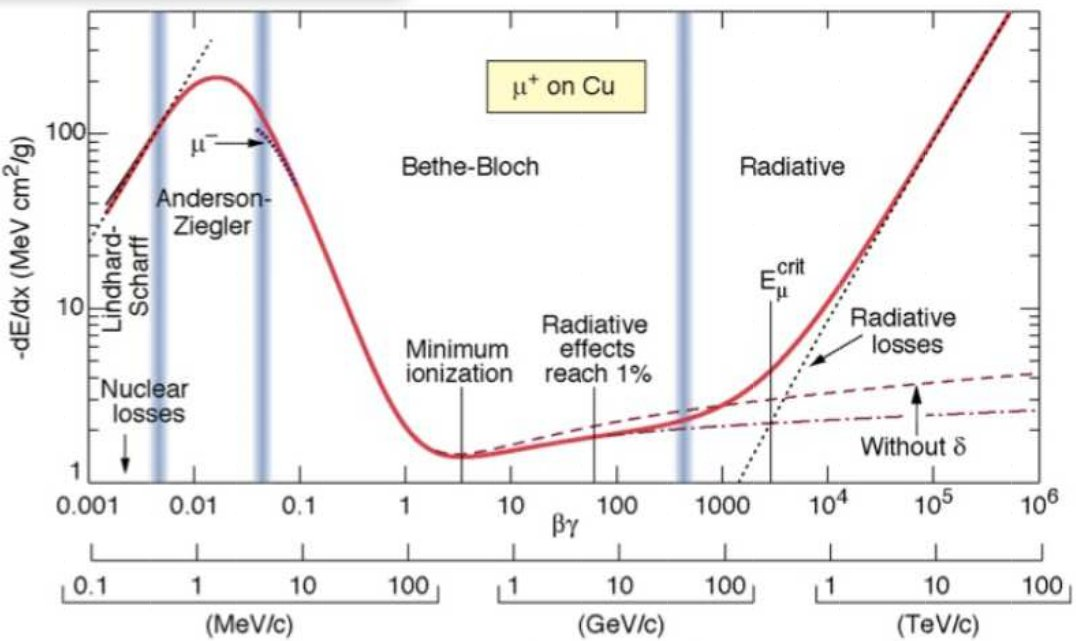
\includegraphics[width=0.5\textwidth]{bethebloch.jpg}
 	\caption{Energieverlust von Myonen in Kupfer}
 	\label{myonenInKupfer}
\end{figure}

\begin{figure}
	\centering
	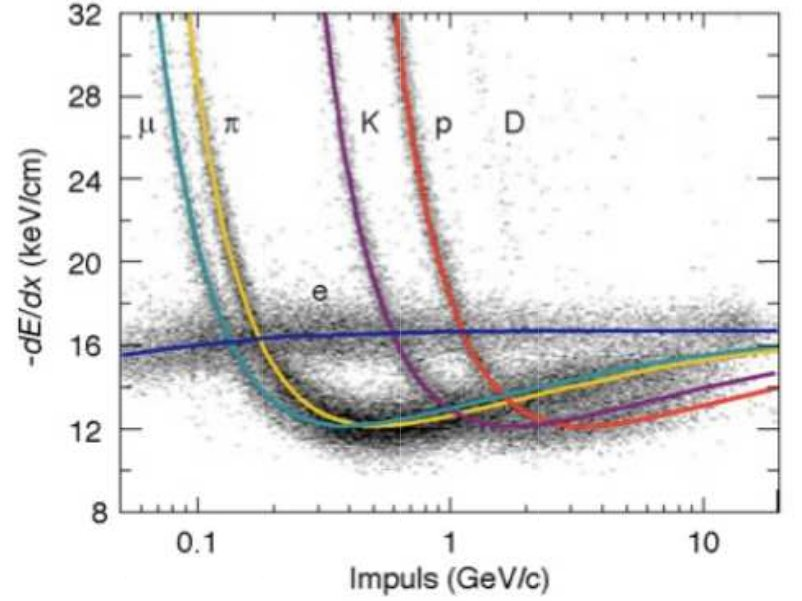
\includegraphics[width=0.5\textwidth]{bethebloch2.jpg}
	\caption{$\frac{dE}{dx}$-Kurven für verschiedene Teilchen (gemessen in der
	PEP4/9-TPC)}
	\label{}
\end{figure}
 
 Beachte: $\frac{dE}{dx}$ für "`schwere"' Teilchen (z.B. $\alpha$) wird in diesem Impulsbereich gut
 durch die Bethe-Bloch-Formel beschrieben. Der Energieverlust durch Ionisation und Anregung von
 Targetelektronen dominiert. $\frac{dE}{dx}$ für Elektronen/Positronen folgt jedoch nicht der
 Bethe-Bloch-Formel!
 
 \FloatBarrier
% 			\subsubsection{Bethe-Bloch-Formel}
% 				Zur klassischen Herleitung der Bethe-Bloch-Formel betrachten wir den Energieverlust $\frac{dE}{dx}$
eines schweren (d.h. $m>>m_e$), geladenen Teilchens durch Streuung an einem Hüllenelektron eines
Targetatoms.
\\
Dabei gelten folgende Annahmen:
\begin{itemize}
  \item das Hüllenelektron ist in Ruhe (Vernachlässigung der Bahnbewegung und des Rückstoßes),
  \item der Energieübertrag ist sehr viel größer als die Bindungsenergie eines Hüllenelektrons.
\end{itemize}


{\Huge ZEICHNUNG}

Der Impulsübertrag ist das Zeitintegral der durch das elektrische Feld des Projektils auf das
Target einwirkenden Kraft. Für die longitudinalen bzw. transversalen Komponenten des E-Feldes gilt

\[E_l(-x)=-E_l(x)~~~~~~~~~~~~~~~~~~~E_t(-x)=E_t(x)\]

d.h. nur der Transversalanteil ist wichtig, die longitudinalen Komponenten im Impulsübertrag heben
sich auf. Es gilt daher

\[\Delta p= \int_{-\infty}^{\infty}F\cdot dt = \int_{-\infty}^{\infty}eE_t\cdot dt =
e\int_{-\infty}^{\infty}E_t\frac{dt}{dx}\cdot dx
=e\int_{-\infty}^{\infty}E_t\frac{1}{v}\cdot dx
=\frac{e}{v}\int_{-\infty}^{\infty}E_t\cdot dx\]

Mit Gauß $\int_{-\infty}^{\infty}E_t2\pi bdx=4\pi ze$ folgt

\[\Delta p = \frac{2ze^2}{vb}\]

und somit für den Energieübertrag

\[\Delta E=\frac{\Delta p^2}{2m_e}=\frac{2z^2e^4}{m_ev^2b^2} .\]

Eine Elektronendichte von $n_e$ ergibt daher einen Energieverlust von 

\[-dE(b)=\Delta E(b)n_edv=\frac{2z^2e^4}{m_ev^2b^2}n_e2\pi b db dx\]

Nach der Integration von $b_min$ bis $b_max$ erhält man daraus:

\[-\left(\frac{dE}{dx}\right)=\frac{4\pi z^2
e^4}{m_ev^2}n_e\text{ln}\left(\frac{b_{\text{max}}}{b_{\text{min}}}\right)\]

Nun müssen nur noch $b_{\text{min}}$ bis $b_{\text{max}}$ abgeschätzt werden. $b_{\text{min}}$ wird über das
kinematische Limit abgeschätzt: Eine frontale Kollision liefert den maximalen Energieübertrag

\[\Delta E_{\text{max}}=\frac{1}{2}m_e(2v)^2\gamma^2.\]

Mit der oben abgeleiteten Beziehung

\[\Delta E(b)=\frac{2z^2e^4}{m_ev^2b^2}\overset{!}{=}\Delta E_{\text{max}}\]

ergibt sich daraus:

\[b_{\text{min}}=\frac{ze^2}{\gamma m_e v^2}.\]

Die Abschätzung von $b_{\text{max}}$ folgt aus der "`adiabatischen Invarianz"': Die Targetelektronen
sind in Atomen gebunden und "`umkreisen"' die Atomkerne mit einer mittleren Orbitalfrequenz
$\overline{\nu}$. Damit ein Energieübertrag stattfindet, muss die Zeitdauer der Störung, $\Delta t$,
kürzer sein als die Periodendauer $\tau$:

\[\Delta t=\frac{b}{\gamma v} \le \tau =\frac{1}{\overline{\nu}}\]

Daraus folgt

\[b_{\text{max}}=\frac{\gamma v}{\overline{\nu}}.\]

Jetzt führen wir noch eine Größe for die Elektronen-Dichte des Target-Materials ein:

\[n_e=N_A\cdot \rho\cdot \frac{Z}{A}\]

mit der Avogadrozahl $N_A$, der Targetdichte $\rho$, der Ordnungszahl $Z$ und der Massenzahl $A$.
Einsetzen der Grenzen für den Stoßparameter in die Formel und Substitution von $n_e$ führt zu

\[-\left(\frac{dE}{dx}\right)_{\text{coll}} = \frac{4\pi z^2e^4}{m_ev^2}N_A\cdot \rho
\frac{Z}{A}\cdot\text{ln}\left(\frac{\gamma^2 m_e v^3}{2e^2\overline{\nu}}\right), \]

was der klassischen Formel von Bohr entspricht. Diese beschreibt den Energieverlust für schwere
Teilchen (Protonen, $\alpha$-Teilchen,\ldots) durch Anregung und Ionisation. Für leichte Teilchen
müssen Quanteneffekte berücksichtigt werden.
\\
Die quantenmechanische Rechnung führt zur Bethe-Bloch(-Sternheimer)-Formel:

\[-\left(\frac{dE}{dx}\right)_{\text{coll}} = 2\pi N_A r_e^2 m_e c^2 \rho \frac{Z}{A}
\frac{z^2}{\beta^2}\left[ \text{ln} \left( \frac{2m_e c^2 \gamma^2 \beta^2 W_{\text{max}}}{I^2}
\right) -2\beta^2 -\delta -2\frac{c}{z} \right]\]

mit 

\[\beta =
\frac{v}{c},~~~~~~~~~~~~\gamma=\frac{1}{\sqrt{1-\beta^2}}~~~~~~~~~~~~
r_e=\frac{1}{4\pi\epsilon_0}\cdot\frac{e^2}{m_e c^2}\]

sowie
\begin{description}
\item[$z$]Ladung des einfallenden Teilchens
\item[$Z, A$] Ordnungs- und Massenzahl des Targets
\item[$\rho$] Targetdichte
\item[$N_A$] Avogradozahl
\item[$I$] mittleres Ionisationspotential (Materialkonstante des Targets)
\item[$W_{\text{max}}$] max. Energieübertrag in einer Einzelkollision
\item[$\delta$] Dichtekorrektur (Polarisationseffekt, $\delta \approx 2\text{ln}(\gamma)+K$)
\item[$c$] Schalenkorrektur (wichtig für kleine Projektilgeschwindigkeiten)
\end{description}


Anmerkungen zur Bethe-Bloch-Formel:
\begin{itemize}
  \item sie beschreibt den Energieverlust sehr gut im Bereich $0,1 < \gamma\beta < 100$;
  \item es gibt drei Bereiche:
  			\begin{itemize}
  			  \item bei niedrigen Energien gibt es einen Abfall bis zu einem Minimum (bei $\gamma\beta$
  			  ca. 3-3,5), Teilchen an diesem Punkt sind minimal ionisierende Teilchen;
  			  \item danach beginnt ein logarithmischer Anstieg mit zunehmender Teilchenenergie, der
  			  sogenannte "`relativistische Anstieg"';
  			  \item bei hohen Energien wird das Fermi-Plateau erreicht: durch Polarisationseffekte erreicht
  			  der Energieverlust  einen Sättigungswert (Dichtekorrektur);
  			  \end{itemize}
  \item beim Energieverlust handelt es sich um einen statistischen Vorgang.
\end{itemize}

Die Bethe-Bloch-Formel beschreibt den mittleren Energieverlust durch Ionisation und Anregung. Sie
gilt für alle geladenen Teilchen außer Elektronen und Positronen. Für diese muss die Gleichheit der
Massen und die Ununterscheidbarkeit der Stoßpartner berücksichtigt werden. Unsere Ableitung
unterscheidet sich von der Bethe-Bloch-Formel numerisch durch einen Faktor 2, was durch eine
mangelhafte Berücksichtigung von Fernstößen zustande kommt. Für die quantenmechanische Beschreibung
des Energieverlustes gibt es verschiedene Varianten der $\frac{dE}{dx}$-Formel, was an der
unterschiedlichen Parametrisierung der Fernstöße, d.h. jenes Energieverlustes, bei dem die Bindung
der Elektronen in den Atomhüllen nicht vernachlässigbar ist.
\\
Meist wird der Energieverlust pro Wegstrecke $\frac{1}{\rho}\frac{dE}{dx}$ angegeben, wobei $\rho$
die Dichte in $\frac{\text{g}}{\text{cm}^3}$ ist. $\frac{1}{\rho}\frac{dE}{dx}$ ist für ein MIP nur
schwach vom Absorbermaterial abhängig und beträgt ca. 

\[2 \text{MeV}\frac{\text{cm}^2}{\text{g}}.\]
% 			\subsubsection{Landau-Verteilung}
% 				\FloatBarrier
Wie kann die Energieverteilung des Energieverlustes für ein gegebenes "`$\beta\cdot\gamma$"' beschrieben
werden? Der Energieverlust ist ein statistischer Prozess mit einer asymmetrischen
Verteilungsfunktion, da Kollisionen mit kleinem Energieübertrag wahrscheinlicher sind als solche
mit großen Energieübetrag.

\begin{figure}
	\centering
	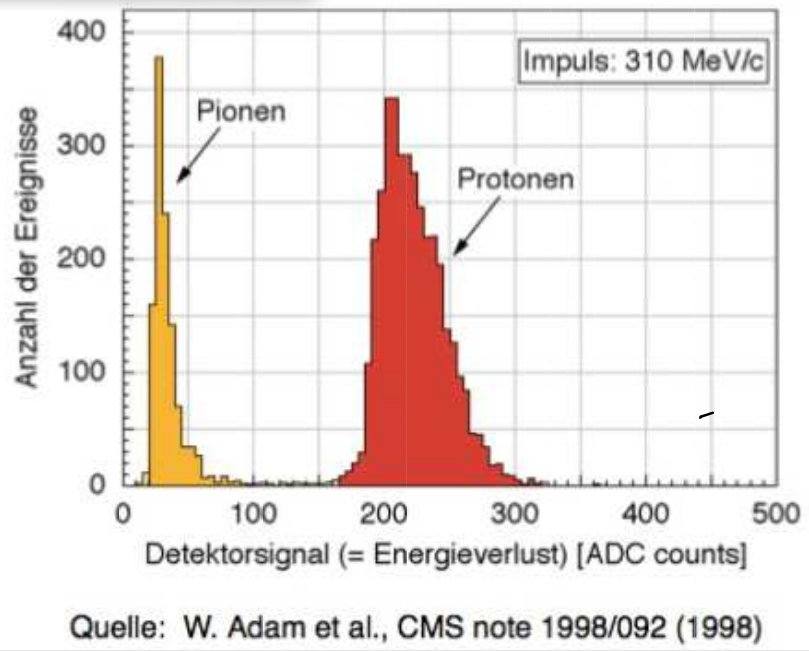
\includegraphics[width=0.5\textwidth]{landau.jpg}
	\caption{Die Energieverteilung des Energieverlustes ist eine Landau-Verteilung.}
	\label{}
\end{figure}

Der Ausläufer bei hohen Energieüberträgen kommt von (selten auftretenden) Kollisionen mit kleinen
Stoßparametern, wobei Elektronen mit großen Ener\-gien (keV), sogenannte $\delta$-Elektronen,
freigesetzt werden. Die Asymmetrie kommt daher, dass der mittlere Energieverlust höher
ist als der wahrscheinlichste Energieverlust.
\\
Bei dünnen Absorbern wird der Energieverlust durch eine Landau-Verteilung beschrieben, bei dicken
Absorbern geht diese über in eine Gauß-Verteilung.

\FloatBarrier
% 			\subsubsection{Bragg-Kurve}
% 				Wie tief dringen Teilchen in das Detektormaterial ein? Man kann für jede
Projektil/Target-Kombination nur eine mittlere Eindringiefe angeben. Der Energieverlust eines
Projektils in Anhängigkeit von der Eindringtiefe wird durch die Bragg-Kurve beschrieben. Mit
Eindringen in die Materie wird das Projektil langsamer, der Energieverlust steigt an
(Bethe-Bloch). Die Reichweite $R$ enthält man aus der Integration des Energieverlustes entlang des
Weges, wobei $\frac{dE}{dx}$ hierbei eine Funktion von $E$ ist. Bei ionisierender Strahlung kommt es
am Ende der Reichweite wegen $\frac{1}{\beta^2}$-Verhalten zu einer besonders hohen Dichte der
deponierten Energie.

\[dE= \frac{dE}{dx}(E)dx~~~~~~~~~~\Rightarrow~~~~~~~~~~dx
=\frac{dE}{dE/dx}~~~~~~~~~~\Rightarrow~~~~~~~~~~ R=\int_{E_c}^{M} \frac{dE}{dE/dx}  \]

Der größte Ionisationsverlust findet nahe am Ende der Spur statt (Bragg-Peak).



% Absorptionsprozesse (mit $dN=8\mu dx$) führen zu einem exponentiellen Abfall der Teilchenzahl.

% \begin{figure}
% \begin{minipage}{0.45\textwidth}
% 
% \end{minipage}
% \begin{minipage}{0.45\textwidth}
% 
% \end{minipage}
% \caption{bla}
% \end{figure} 

\begin{figure}[htbp]
	\begin{minipage}[b]{0.5\textwidth}
		\begin{figure}[H]
		\centering
		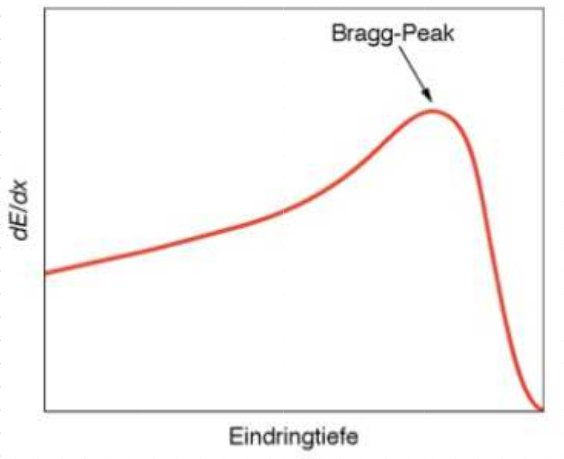
\includegraphics[width=\textwidth]{bragg.jpg}
		\end{figure}
	\end{minipage}
	\hfill
	\begin{minipage}[b]{0.5\textwidth}
		\begin{figure}[H]
		\centering
		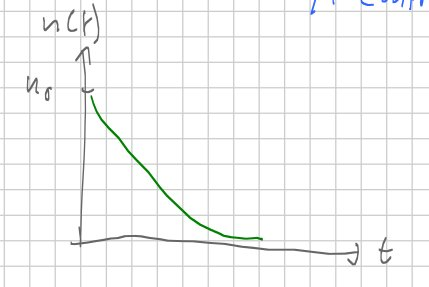
\includegraphics[width=\textwidth]{expabfall.jpg}
		\end{figure}
	\end{minipage}
	\caption{b}
	\label{rekristall} 
\end{figure}
% 			\subsubsection{Delta-Elektronen}
% 				\FloatBarrier

Die kinetischen Energien der Elektronen ist proportional zu $\frac{1}{\Delta E^2}$.
$\Delta E$ ist dabei der Energieübertrag des Projektils auf das Hüllenelektron.

\[\frac{d\sigma}{d\Delta E} = \frac{2\pi\cdot z^2\cdot \alpha^2\cdot \hbar^2}{\beta^2\cdot m_e}\cdot
\frac{1}{\Delta E^2}
\]

Die Ausläufer dieser Verteilung gehen bis $\Delta E_\text{max}$,

\[\Delta E_\text{max} = \frac{2m_e\cdot c^2\cdot \beta^2\cdot \gamma^2}{1+ 2\,\gamma\,
\frac{m_e}{M}+\left( \frac{m_e}{M} \right)^2}\]

mit den Grenzwerten
\begin{itemize}
  \item $\gamma\rightarrow\infty$: $\Delta E_\text{max} \rightarrow \gamma Mc^2$
  \item $m_e = M$: $\Delta E_\text{max} =m_e c^2 (\gamma -1) = E- m_e c^2$ \\
  		Die komplette Energie wird auf das Hüllenelektron übertragen.
\end{itemize}

Für relativistische Teilchen ($\gamma >> 1$) kann $\Delta E_\text{max}$ sehr groß werden und
Elektronen mit Energien von einigen keV hervorbringen. In Detektoren mit hoher Granularität und Ortsauflösung (z.B.
Blasenkammern) können sie als sogenannte Delta-Elektronen nachgewiesen werden.
\\
Seltene Abstrahlung hoher Energie führt auch zu größeren Fluktuationen in $\frac{\mathrm{d}E}{\mathrm{d}x}$-Messungen
zur Teilchenidentifikation und damit zu einer schlechteren Auflösung. Auch bei Detektoren mit
geringer Granularität führt die Abstrahlung von Delta-Elektronen zu einer schlechteren
Ortsauflösung.
\\
Eine genaue Rechnung zeigt: 

\[\Delta E (\Theta) = \frac{2\,m_e}{\text{tan}^2\Theta} \]

Größere Abstrahlungswinkel führen zu kleineren Energien der Delta-Elektronen, was in einer
geringeren Reichweite resultiert.
\FloatBarrier
% 			\subsubsection{Energieverlust von Elektronen und Positronen}
% 				\FloatBarrier
Elektronen und Positronen haben durch ihre geringe Masse eine Sonderstellung
($m_{e^{\pm}} \approx 511$~keV/c$^2$, $m_{\mu} \approx 106$~MeV/c$^2$). Zusätzlich zum Energieverlust durch Ionisation und
Anregung hat daher der Energieverlust durch Bremsstrahlung eine größere Bedeutung:

\[-\left(\frac{\mathrm{d}E}{\mathrm{d}x}\right)_{\text{tot}} = -\left(\frac{\mathrm{d}E}{\mathrm{d}x}\right)_{\text{coll}}
-\left(\frac{\mathrm{d}E}{\mathrm{d}x}\right)_{\text{rad}} \]

Beim Energieverlust durch Ionisation und Anregung muss die Bethe-Bloch-Formel wegen der geringen
Masse modifiziert werden, aber auch, da eine Kollision zwischen quantenmechanisch nicht
unterscheidbaren Teilchen stattfindet. Die Ionisationsverluste steigen logarithmisch mit $E$ und
linear mit $Z$, die Bremsstrahlungsverluste dagegen in etwa linear mit $E$ und quadratisch mit $Z$.
Für hohe Energien (> 1~GeV) ist die Bremsstrahlung der dominierende Prozess.

\begin{figure}
	\centering
	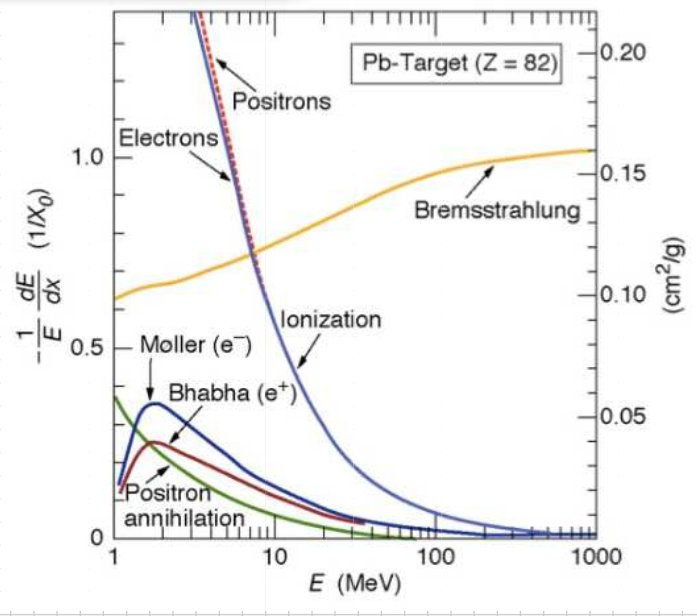
\includegraphics[width=0.5\textwidth]{energieverlust.jpg}
	\caption{}
	\label{}
\end{figure}

% Elektronen/Positronen Streuung an Targetelektronen fällt unter Ionisation, wenn der Energieübertrag
% pro Kollision unter 0,255~MeV liegt und unter M\o ller-Streuung (Bhabha-Streuung), wenn er darüber
% liegt.

\FloatBarrier
% 			\subsubsection{Bremsstrahlung}
% 				\FloatBarrier
Bremsstrahlung wird emittiert, wenn (hochenergetische) geladene Teilchen in einem äußeren
elektrischen Feld abgelenkt werden, beispielsweise im Coulomb-Feld eines Atomkerns oder eines
Hüllenelektrons des Targets.
\\
Die zughörigen Feyman-Diagramme niedrigster Ordnung:
\\
\\

\begin{figure}[H]
	\begin{minipage}[b]{0.5\textwidth}
		\begin{figure}[H]
		\centering
		\includesvg[svgpath=bilder/1-1/]{feynman1}
		\end{figure}
	\end{minipage}
	\hspace{5mm} 
	\begin{minipage}[b]{0.5\textwidth}
		\begin{figure}[H]
		\centering
		\includesvg[svgpath=bilder/1-1/]{feynman2}
		\vspace{3mm}
		\end{figure} 
	\end{minipage} 
\end{figure}




% \begin{fmffile}{diagram}
% \begin{fmfgraph}(40,25)
% \fmfleft{i1,i2}
% \fmfright{o1,o2}
% \fmf{photon}{i1,v1,o1}
% \fmf{fermion}{i2,v2,o2}
% \fmf{photon}{v1,v2}
% \end{fmfgraph}
% \end{fmffile} 


% \begin{fmffile}{hilde}
% \begin{fmfgraph}(40,25)
% \fmfleft{i1,i2}
% \fmfright{o1,o2}
% \fmf{fermion}{i2,v2,v1,o1}
% \fmf{photon}{i1,v1}
% \fmf{photon}{v2,o2} 
% \end{fmfgraph}
% \end{fmffile} 


% 
% \begin{minipage}[t]{0.3\textwidth}
% \begin{fmffile}{hubert}
% \begin{fmfgraph*}(100,100)
% \fmfleft{i1,i2}
% \fmfright{o1,o2}
% \fmf{fermion}{i1,v1,v2,o2}
% \fmf{photon}{i2,v2}
% \fmf{photon}{v1,o1}
% \fmflabel{v1}{v1}
% \fmflabel{v2}{v2}
% \fmflabel{$e^-(p)$}{i1}
% \fmflabel{$\gamma(k)$}{i2}
% \fmflabel{$\gamma(k)$}{o1}
% \fmflabel{$e^-(p)$}{o2}
% \end{fmfgraph*}
% \end{fmffile}
% \end{minipage}
% \begin{minipage}[t]{0.3\textwidth}
% \begin{fmffile}{hubert}
% \begin{fmfgraph}(100,100)
% \fmfleft{i1,i2}
% \fmfright{o1,o2}
% \fmf{fermion}{i1,v1,v2,o2}
% \fmf{photon}{i2,v2}
% \fmf{photon}{v1,o1}
% \fmflabel{$v_1$}{v1}
% \fmflabel{$v_2$}{v2}
% % \fmflabel{$e^-(p)$}{i1}
% % \fmflabel{$\gamma(k)$}{i2}
% % \fmflabel{$\gamma(k)$}{o1}
% % \fmflabel{$e^-(p)$}{o2}
% \end{fmfgraph}
% \end{fmffile}
% \end{minipage}


\subsubsection*{Energieverlust durch Bremsstrahlung}

Für hohe Energien kann der Energieverlust durch Bremsstrahlung angenähert weren durch:

\[-\left(\frac{\mathrm{d}E}{\mathrm{d}x}\right)_{\text{rad}} = 4\,\alpha\cdot \rho\cdot N_A \cdot
\frac{Z(Z+1)}{A} \cdot z^2\cdot \left(\frac{1}{4\,\pi\cdot \epsilon_0}\cdot \frac{e^2}{m\cdot c^2}
\right)^2 \cdot E\cdot \text{ln}(183\cdot Z^{-1/3}) \]

Der Beitrag $Z^2$ kommt von der Ablenkung im Feld des Kerns mit der Ladung $Z\cdot e$, der Beitrag
$Z$ von der Ablenkung im Feld der $Z$ Hüllenelektronen jeweils mit Ladung $-e$. Hierbei wird nicht
berücksichtigt, dass die Hüllenelektronen das Feld des Atomkerns teilweise abschirmen und die Formel
daher nur für große $E$ gültig ist.
\\
Beachte: Bereits für das zweitleichteste Teilchen, das Myon, ist der Bremsstrahlungsverlust 40.000
mal kleiner als für das Elektron. Es gilt

\[-\left(\frac{\mathrm{d}E}{\mathrm{d}x}\right)_{\text{rad}} \sim E~~~~~~\text{und}~~~~~
-\left(\frac{\mathrm{d}E}{\mathrm{d}x}\right)_{\text{rad}} \sim \frac{1}{m^2}.\]

\subsubsection*{Kritische Energie $E_c$}

Die kritische Energie ist jene Energie eines Projektils, bei welcher der Energieverlust durch
Strahlung gleich dem Energieverlust durch die Kollision ist:

\[-\left(\frac{\mathrm{d}E}{\mathrm{d}x}\right)_{\text{rad}} \bigg|_{E_c} = -\left(\frac{\mathrm{d}E}{\mathrm{d}x}\right)_{\text{coll}}
\bigg|_{E_c}  \]

$E_c$ ist abhängig von der Teilchenart des Projektils und vom Targetmaterial (wenn nicht anders
gekennzeichnet, beziehen sich Literaturwerte auf Elektronen). Die kritische Energie skaliert in etwa
mit dem Quadrat der Projektilmasse. Um nun beispielsweise die kritische Energie für Myonen zu
erhalten, verwendet man:

\[E_c^\mu = E_c^e \left( \frac{m_\mu}{m_e} \right)^2 \]

Zur groben Abschätzung von $E_c$ sind diverse Näherungen gegeben, z.B.

\[E_c = \frac{800}{Z+1{,}2}~\text{MeV} \]

oder für Festköper

\[E_c = \frac{610}{Z+1{,}24}~\text{MeV} \]

oder für Gase

\[E_c = \frac{710}{Z+0{,}92}~\text{MeV} \]


Die bekannten Zahlenwerte für $E_c$ schwanken relativ stark:

\begin{figure}[H]
	\centering
	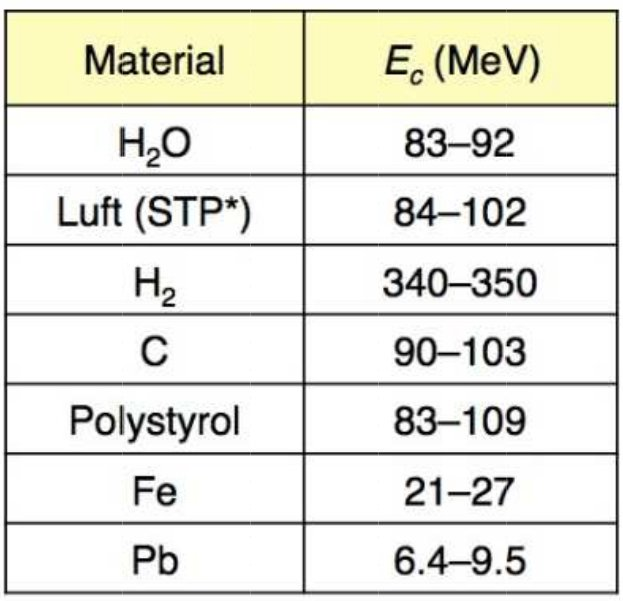
\includegraphics[width=0.5\textwidth]{tabelle1.jpg}
\end{figure}

\subsubsection*{Strahlungslänge $\chi_0$}

Die Strahlungslänge ist jene Strecke, in der die Energie des Projektils durch Strahlungsverluste um
einen Faktor $\frac{1}{e}~(\approx63{,}2\,\%)$ kleiner wird:

\[E(x)=E_0\cdot e^{-\frac{x}{\chi_0}}.\]

Diese Beziehung ist nur sinnvoll für Energien größer als $E_c$. Die Literaturwerte für $\chi_0$
beziehen sich dabei stets auf Elektronen, für andere Teilchen skaliert die Strahlungslänge mit dem
Quadrat der Projektilmasse (ebenso wie bei $E_c$).
\\
Die oben gegebene Formel für die Bremsstrahlung führt für Elektronen auf eine Strahlungslänge
von 

\[\frac{1}{\chi_0}=4\,\alpha\cdot \rho\cdot N_A \cdot\frac{Z(Z+1)}{A}\cdot
r_e^2\cdot\text{ln}\left(183\cdot Z^{-1/3}\right)\]

\[\text{Näherungsformel:}~~\chi_0\bigg[\frac{\text{g}}{\text{cm}^2}\bigg] \approx
180~\frac{A}{Z^2}\] 

Meist werden Materialdicken von Targets in Einheiten von $\chi_0$ angegeben, womit der
Strahlungsverlust pro Targetdicke dann materialunabhängig ist. Genauso wird die Strahlungslänge -
analog zur Energieverlustrate - auf die Targetdichte bezogen ($\rho \chi_0\rightarrow\chi_0$) und
folglich in [g/cm$^2$] angegeben:

\begin{figure}[H]
	\centering
	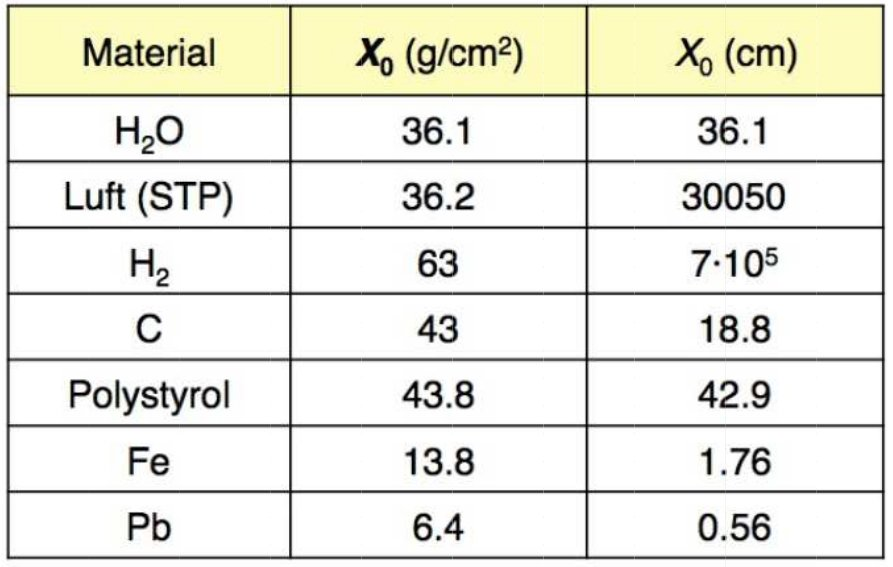
\includegraphics[width=0.5\textwidth]{tabelle2.jpg}
\end{figure}

\FloatBarrier
% 			\subsubsection{\v{C}erenkov-Strahlung}
% 				\v{C}erenkov-Strahlung wird emittiert, wenn die Geschwindigkeit $v$ eines Teilchens größer ist als
die Lichtgeschwindigkeit in dem vom Teilchen durchquerten Material:

\begin{figure}[H]
	\centering
	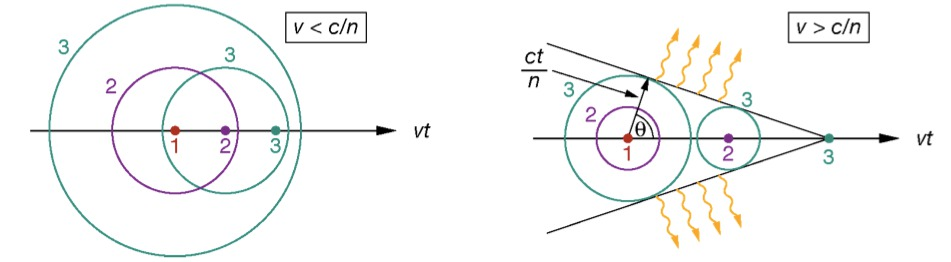
\includegraphics[width=0.8\textwidth]{cerenkov.jpg}
	\caption{Veranschauulichung der Entstehung von \v{C}erenkov-Strahlung. Links $v<c/n$, rechts $v>cn$
	(elektromagnetische Schockwelle) mit $c=$ Vakuumlichtgeschwindigkeit und $n=$ Brechungsindex. }
\end{figure}

Bewegt sich ein geladenes Teilchen durch ein dielektrisches (nichtleitendes) Medium, kommt es zu
einer kurzzeitigen Polarisierung der Atome längs der Flugbahn durch dessen Ladung. Dabei werden
elektromagnetische Wellen erzeugt. Im Normalfall inteferieren die Wellen destruktiv mit den Wellen
von benachbarten Atomen. Ist das Teilchen jedoch schneller als das Licht in diesem Medium, können
sich die Wellen nicht mehr gegenseitig auslöschen. Es entsteht eine gemeinsame kegelförmige
Wellenfront, die \v{C}erenkov-Strahlung.
\\
Die kohärente Wellenfront hat konische Form und wird unter einem Winkel von 

\[\text{cos}\,\Theta_c=\frac{1}{\beta\cdot n}~~~~~\text{mit}~~\beta=\frac{v}{c}\]

abgestrahlt. \v{C}erenkov-Strahlung ist nur für ca 1\% des Energieverlustes eines Teilches
verantwortlich. Die Zahl der pro Weglänge $L$ abgestrahlten Photonen beträgt

\[\frac{dN_{ph}}{dL}= 2\pi\cdot\alpha\cdot z^2 \int_{\lambda_2}^{\lambda_1}
\frac{\overbrace{1-1/(\beta^2n^2)}^{\text{sin}^2\,\Theta}}{\lambda^2}\,\mathrm{d}\lambda\]

mit der Ladung $z$ des Teilchens und der Wellenlänge $\lambda$ der Strahlung. 
\\
Unter der Annahme, dass $n(\lambda)$ im entsprechenden Wellenlängenbereich konstant ist, gilt

\[\frac{dN_{ph}}{dL}= 2\pi\cdot\alpha\cdot z^2 \, \frac{1-1/\beta^2n^2}{\lambda}\]

Die Zahl der abgestrahlten Photonen nimmt mit kleinerer Wellenlänge wie 1/$\lambda$ zu.
% 			\subsubsection{Übergangsstrahlung}
% 				\FloatBarrier
Übergangsstrahlung tritt auf, wenn ein geladenes Teilchen die Grenzfläche zweier
Materialien mit unterschiedlicher Dielektrizitätskonstante $\epsilon$ durchquert.
\\
Bei Material mit niedrigem $\epsilon$ ist die Polarisation des Materials klein, das elektrische Feld
der bewegten Ladung hat eine große räumliche Ausdehnung. Bei Material mit hohem $\epsilon$ hingegen
ist die Polarisation der Materials groß, das elektrische Feld der bewegten Ladung hat somit eine
geringe räumliche Ausdehnung. Die plötzliche Umverteilung der Ladungen an der Grenzfläche und die
daraus resultierende schnelle Änderung des elektrischen Feldes ist die Ursache der
Übergangsstrahlung.
\\
Übergangsstrahlung wird hauptsächlich als Röntgenstrahlung emittiert. Die Emissionsrichtung liegt in
der Bewegungsrichtung des Projektils innerhalb eines Konus mit dem Öffnungswinkel

\[\text{cos}\,\Theta_t \approx \frac{1}{\gamma}~~~~~\text{mit}~~~\gamma=\frac{1}{\sqrt{1-\beta^2}} 
\]

Tritt ein Teilchen mit der Ladung $z\cdot e$ vom Vakuum in ein Medium mit der Plasmafrequenz
$\omega_p$ über, so liegt die als Übergangsstrahlung emittierte Energie bei

\[E_t = \frac{1}{3}\, \alpha\cdot z^2\cdot \gamma\cdot \hbar\cdot\omega_p. \]

Mittels Energiemessung der Übergangsstrahlung kann man $\gamma$ und somit die
Projektilgeschwindigkeit messen. Für eine typische Photonenergie von $\gamma\cdot
\hbar\cdot\omega_p/4$ ist die mittlere Anzahl von emittierten Photonen pro Grenzfläche
(=~Quantenausbeute) ungefähr

\[ \langle N \rangle = \frac{2}{3}\,\alpha\cdot z^2~~~~~\text{mit}~~~~\alpha\sim \frac{1}{137}.  \]

\FloatBarrier

\graphicspath{{bilder/1-2/}}
	\subsection{Wechselwirkung von Photonen}
		\FloatBarrier
In Teilchendetektoren finden folgende Wechselwirkungen von Photonen mit Materie statt:

\begin{figure}[H]
	\centering
	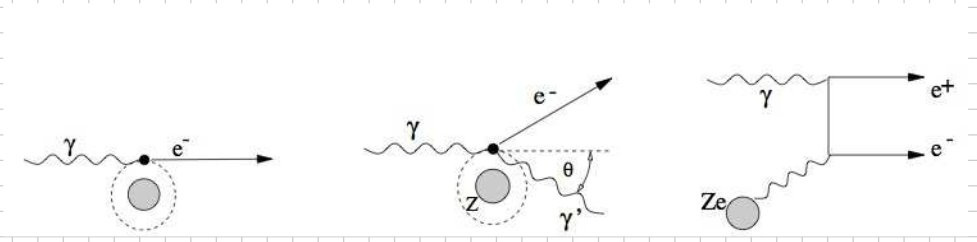
\includegraphics[width=\textwidth]{1-wewiMitMaterie.jpg}
\end{figure}

Bei niedrigen Energien überwiegt der Photoeffekt, bei dem das Photon seine gesamte Energie auf ein
Hüllenelektron überträgt. Bei mittleren Energien kommt der Compton-Effekt hinzu, der eine elastische
Streuung eines Photons an einem Hüllenelektron beschreibt. Bei hohen Energien überwiegt schließlich
die Paarbildung, bei der ein Photon im Kernfeld in ein $e^+e^-$-Paar konvertiert.

\begin{figure}
	\centering
	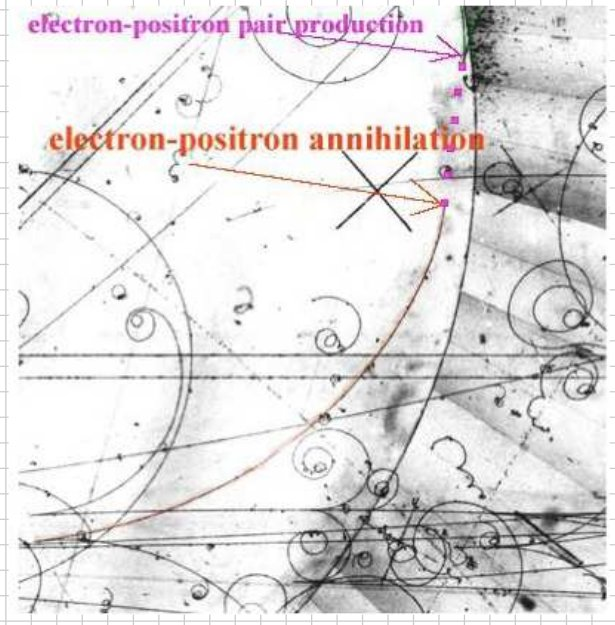
\includegraphics[width=0.5\textwidth]{2-pairProduction.jpg}
\end{figure}

Bei sehr niedrigen Photonenergien kommt es zur Thomson- und Rayleighstreuung (s. Kap.
\ref{thomsonrayleigh}).
\\
Für Photonen relevante Energiebereiche sind  

\begin{itemize}
  \item UV-Licht: eV
  \item Röntgenstrahlung: eV-keV
  \item Gammastrahlung: keV-MeV
\end{itemize}

Ein wichtiger Unterschied zu geladenen Teilchen besteht darin, dass die obigen Prozesse einzelne
Photonen streuen bzw. absorbieren und diese dadurch aus dem Strahl entfernt werden. Die Energie der
Photonen bleibt unverändert (Ausnahme: Compton-Effekt), es kommt nur zu einer Verringerung der
Intensität.

\FloatBarrier
\subsubsection*{Quantitative Beschreibung}

Photonen werden mit einer Wahrscheinlichkeit, die proportional zur Wegstrecke $\mathrm{d}x$ ist,
absorbiert bzw. beim Compton-Effekt gestreut. Wir definieren einen Absorptionskoeffizienten $\mu$,
der die Absorptionswahrscheinlichkeit pro Wegstrecke angibt:

\[ -\frac{1}{N}\cdot\frac{\mathrm{d}N}{\mathrm{d}x}=\mu.\]

Mit der Anzahl $\mathrm{d}N_T$ der Targetteilchen pro Strecke $\mathrm{d}x$ und Fläche $F$ (also
dem Volumen $V$), dem Atomgewicht $A$, der Teilchendichte $n$ und dem Absorptionswirkungsquerschnitt
$\sigma$ erhält man

\[N_T=\frac{\rho\cdot V}{A}\cdot N_A\]
\[\Rightarrow~~~n=\frac{N_T}{V}=\frac{\rho}{A}\cdot N_A\]
\[\Rightarrow~~~-\frac{1}{N}\frac{\mathrm{d}N}{\mathrm{d}x}=\mu=\frac{\mathrm{d}N_T}{\mathrm{d}x}\cdot
\frac{\sigma}{F}=\rho\cdot\frac{N_A}{A}\cdot\sigma=n\cdot\sigma \]

Die mittlere freie Weglänge $\lambda$ ist

\[ \lambda = \frac{1}{\mu}=\frac{1}{n\cdot \sigma} \]

Auch hier sind die auf die Dichte 1 bezogenen Größen in der Literatur zu finden
(Massenabsorptionskoeffizienten). 
\\
Es gilt

\[ \frac{\mu}{\rho}=\frac{N_A}{A}\cdot \sigma \]

\begin{figure}[H]
		\centering
		\includesvg[svgpath=bilder/1-1/]{photonen}
\end{figure}

Die Anzahl der Photonen im Strahl folgt dem Exponentialgesetz

\[N(x)=N_0\cdot e^{-\mu x} \]

\begin{figure}[H]
	\centering
	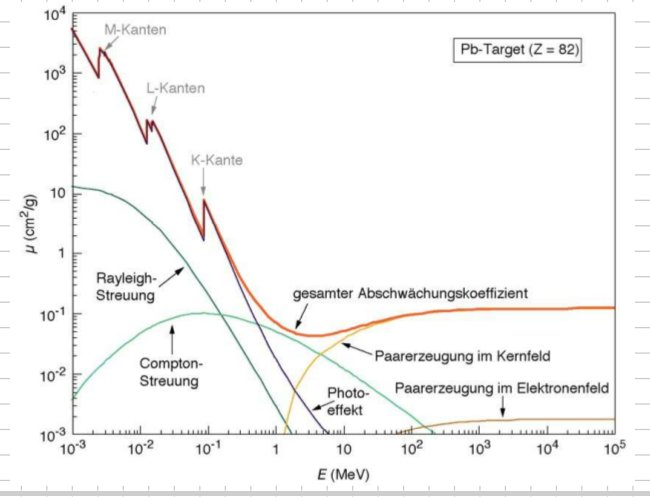
\includegraphics[width=0.5\textwidth]{3-alleEffekte.jpg}
\end{figure}

Abgesehen von einem engen Bereich um etwa $1\,$MeV dominieren Paarbildung und Photoeffekt. Die
Prozesse finden in Abhängigkeit der Energie, aber auch der Kernladungszahl $Z$ des Targets statt. 

\begin{figure}[H]
	\centering
	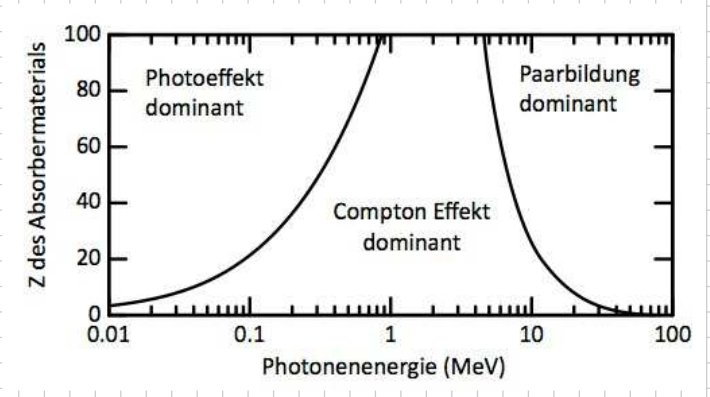
\includegraphics[width=0.5\textwidth]{4-effekteInAbhaengEnergie.jpg}
\end{figure}

Die Abhängigkeiten werden in den folgenden Kapiteln diskutiert. 
\FloatBarrier
			\subsubsection{Thomson- und Rayleigh-Streuung}
				Diese Art der Streuung findet nur bei niederenergetischen Photonen statt. Die Thomson-Streuung
ist die Streuung von Photonen an freien Elektronen im klassischen Limit, wobei

\[ \sigma_0= \frac{8\pi}{3}\cdot r_e^2 \]

Bei der Rayleigh-Streuung streuen die Photonen am gesamten Atom, wobei alle Hüllenelektronen in
kohärenter Form beteiligt sind (kohärente Streuung).
\\
Für beide Prozesse gilt, dass kein Energieübertrag auf das Medium stattfindet. Bei hohen Energien
sind sie vernachlässigbar.
			\subsubsection{Thomson- und Rayleigh-Streuung}
				Beim Photoeffekt wird das Photon von einem Elektron der Atomhülle absorbiert. Das Elektron wird
dabei freigesetzt.
\\
Wegen Impulserhaltung ist dieser Prozess nur im Feld eines Atomkerns möglich, der den Rückstoß 
"`auffängt"'. Freie Elektronen können also kein Photon absorbieren. Die Energie des freiwerdenden
Elektrons ist

\[ E_e=E_\gamma - E_{\text{Bindung}} \]

Der Energieverlauf des Wirkungsquerschnittes für den Photoeffekt folgt aus der Schalenstruktur der
Atome. $\sigma_\text{Photo}$ steigt abrupt an, wenn die Energie $E_\gamma$ ausreicht, um Elektronen
einer "`neuen"' Schale (M, L, K) auszulösen. Für Photonenenergien oberhalb der "`K-Kante"'
dominieren die Elektronen der K-Schale den Photoeffekt. Am größten wird $\sigma_\text{Photo}$ für
die innersten Schalen.
\\
Im mittleren bzw. nicht-relativistischen Energiebereich unter Vernachlässigung der Absorptionskanten
kann man den Wirkungsquerschnitt mithilfe der Bornschen Näherung schreiben als

\[ \sigma_\text{Photo} = 4\sqrt{2} \cdot \alpha^4 \sigma_0 \cdot Z^5 \left(\frac{m_ec^2}{E_\gamma}
\right)^{7/2} \sim \frac{Z^5}{E_\gamma^{\,7/2}} \]

mit dem Thomson-Wirkungsquerschnitt $\sigma_0\approx 0{,}66\,$barn. Für hohe Energien, d.h.
$E_\gamma>>E_{\text{Bindung}}$ in der K-Schale, gilt

\[\sigma_\text{Photo} = \frac{3}{2} \cdot \alpha^4 \cdot\sigma_0 \cdot Z^5\,
\frac{m_ec^2}{E_\gamma} \sim \frac{Z^5}{E_\gamma} \]

Eine allgemeine Abhängigkeit von $\sigma_\text{Photon}$ von $Z$ und $E_\gamma$ kann man schreiben
als

\[ \sigma_\text{Photo} \sim \frac{Z^n}{E_\gamma^m} \]

mit $n=4\ldots5$ und $m=3$ für leichte Elemente und $m=2{,}5$ für schwere Elemente (im
nicht-relativistischen Bereich).

\subsubsection*{Signale im Detektor}

Beim Photoeffekt wird die entstandene Lücke in einer inneren Schale durch Elektronen einer
(nächst-)höheren Schale aufgefüllt. Die freiwerdende Energie wird durch Emission von Photonen oder
Elektronen (Auger-Elektron) abgegeben. Da die Energieüberträge diskret sind, sind folglich auch die
Elektronenenergien diskret. 
\\
Im Photondetektor kann der sogenannte Photopeak beobachtet werden, wenn die gesamte Energie
nachgewiesen wird.  Wenn ein sekundäres Photon mit diskreter Energie den Detektor verlässt, kann
es zur Ausbildung eines zweiten Peaks kommen, dem Escape-Peak (siehe Beispiel Bild
\ref{escapepeak}).

\begin{figure}[H]
	\centering
	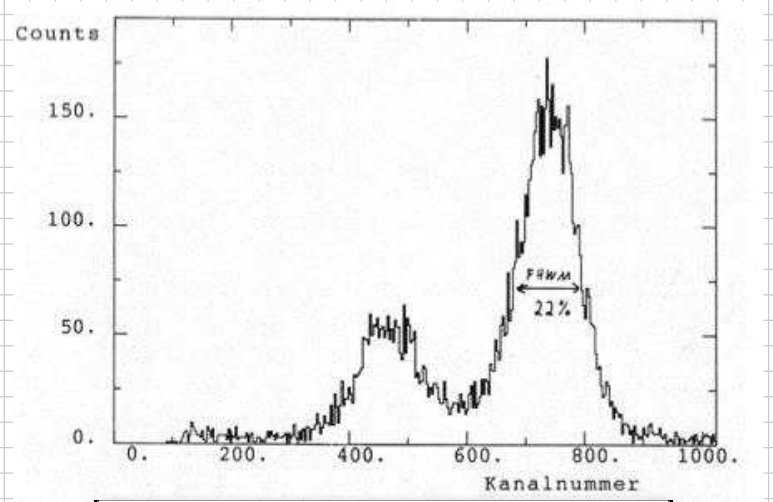
\includegraphics[width=0.5\textwidth]{5-escapePeak.jpg}
	\caption{Beispiel: Test von Proportionalkammern mit einem $^{55}$Fe-Präparat, Linie bei
	$5{,}89\,$keV. Photonen werden im Argongas der Kammer absorbiert, wodurch unterhalb des Photopeaks
	bei etwa $2{,}9\,$keV ein Escape-Peak auftritt.
	}
	\label{escapepeak}
\end{figure}
 
			\subsubsection{Compton-Effekt}
				Der Compton-Effekt beschreibt die Streuung eines Photons an einem quasi-freien Elektron. Dabei ist
die Photonenergie $E_\gamma$ groß im Vergleich zur Bindungsenergie $E_{\text{Bindung}}$ der
Hüllenelektronen, sodass diese vernachlässigt werden kann.

\[ \gamma + \text{Atom} \longrightarrow \gamma + e^- +\text{Ion}\]

Das Photon wird von seiner usprünglichen Bahn abgelenkt und seine Wellenlänge durch den
Energieübertrag auf das Elektron geändert. 

\begin{figure}[H]
	\centering
	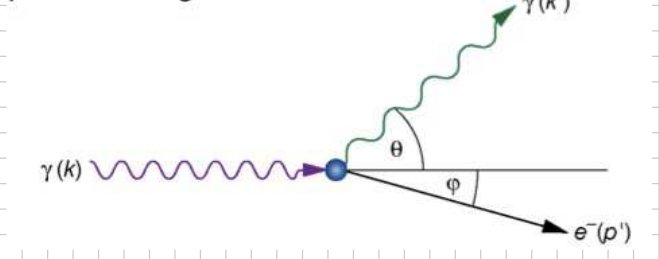
\includegraphics[width=0.5\textwidth]{6-kinematik.jpg}
	\caption{Kinematik des Compton-Effekts	}
	\label{}
\end{figure}

Die Energie des gestreuten Photons lässt sich aus der Kinematik als Funktion des Streuwinkels
berechnen:

\[ E_\gamma' = \frac{E_\gamma}{1+ \frac{E_\gamma}{m_ec^2}\left(1-\text{cos}\,\Theta\right)} \]

Aus der QED und Berechnung der Feynmangraphen erhalten wir die Klein-Nichina-Formel für den
winkelabhängigen Streuquerschnitt eines Photons an einem Elektron (s. Abb. \ref{fgraph2}):

\[ \frac{\mathrm{d}\Theta}{\mathrm{d}\Omega} = \frac{r_e^2}{2
\left[1+\epsilon\left(1-\text{cos}\,\Theta \right) \right]^2} \left(1+\text{cos}^2\,\Theta +
\frac{\epsilon^2\left(1-\text{cos}\,\Theta \right)^2}{1+\epsilon\left(1- \text{cos}\,\Theta \right)}
\right)
\]

mit $\epsilon = \frac{E_\gamma}{m_ec^2}$.

\begin{figure}[H]
	\centering
	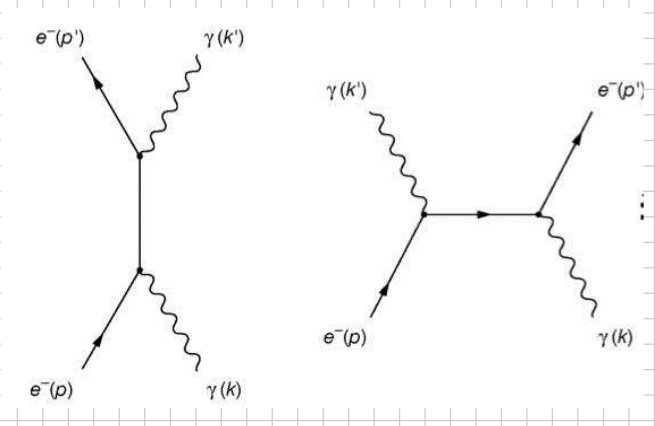
\includegraphics[width=0.5\textwidth]{7-feynmanGraphen.jpg}
	\caption{feynmangraphen???	}
	\label{fgraph2}
\end{figure}

\begin{figure}[H]
	\centering
	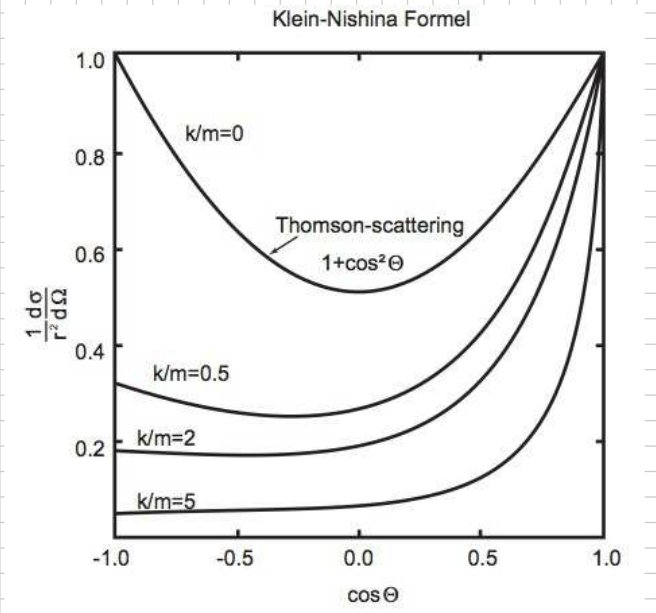
\includegraphics[width=0.5\textwidth]{8-kleinNishinaFormel.jpg}
	\caption{	klein nishina formel ???}
	\label{kleinnishina}
\end{figure}

In Abb. \ref{kleinnishina} ist die Winkelverteilung für die Compton-Streuug zu sehen. Für großen
$E_\gamma$ ergibt sich ein starker Anstieg in Vorwärtsrichtung.
\\
Nach Integration über den Raumwinkel und Summation über alle Elektronen eines Atoms erhält man den
totalen Compton-Wirkungsquerschnitt pro Atom:

\[\sigma_{\text{Compton}} = 2\pi \cdot r_e^2\cdot Z \cdot
\left[\frac{1+\epsilon}{\epsilon}\left( \frac{2(1+\epsilon)}{1+2\epsilon} -
\frac{1}{\epsilon}\,\text{ln}(1+2\epsilon) \right) + \frac{1}{2\epsilon}\,\text{ln}(1+2\epsilon) -
\frac{1+3\epsilon}{(1+2\epsilon)^2} \right] \]

\[\Rightarrow\,\, \sigma_{\text{Compton}} \sim N(e^-) \sim Z  \]

\begin{figure}[H]
	\centering
	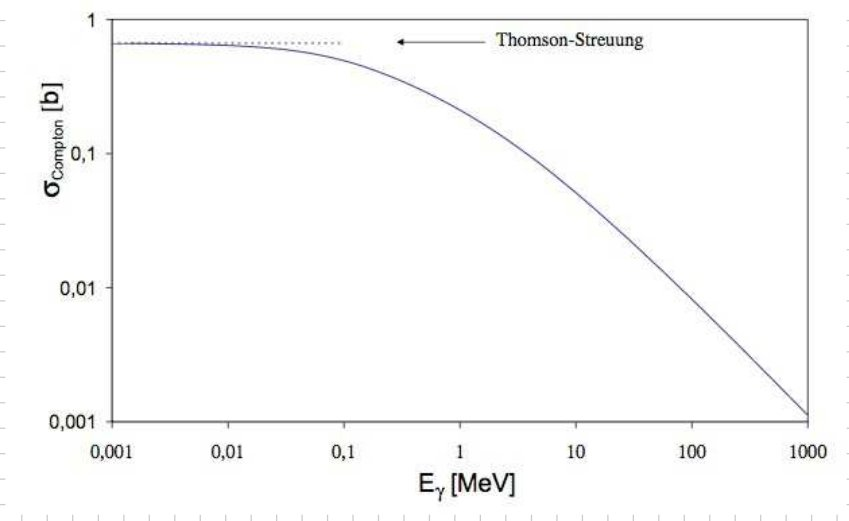
\includegraphics[width=0.5\textwidth]{9-thomsonStreuung.jpg}
	\caption{	comptonwq ???}
	\label{comptonwq}
\end{figure}

Im Detektor wird häufig nur die Energie $E_{\text{kin}}$ des Rückstoßelektrons nachgewiesen,

\[T= E_\gamma -E_\gamma'.  \]

Der Wirkungsquerschnitt hierfür ist

\[\frac{\mathrm{d}\sigma}{\mathrm{d}T} = \frac{\pi\cdot r_e^2}{m_e\cdot c^2\cdot \epsilon^2} \left[
2+ \frac{t^2}{\epsilon^2(1-t)^2} +\frac{t}{1-t}\left(t-\frac{2}{\epsilon} \right) \right] \]

mit $t=\frac{T}{E_\gamma}$.
\\
Die maximalen Elekronenenergie für ein rückwärts-gestreutes Photon (d.h. $\text{cos}\,\Theta=-1$)
ist

\[T_{\text{max}} = E_\gamma\cdot \frac{2\epsilon}{1+2\epsilon}. \] 

Dies wird auch als Compton-Kante bezeichnet und liegt im Energiespektrum des Detektors etwas
unterhalb des Photo-Peaks.

\begin{figure}[H]
	\centering
	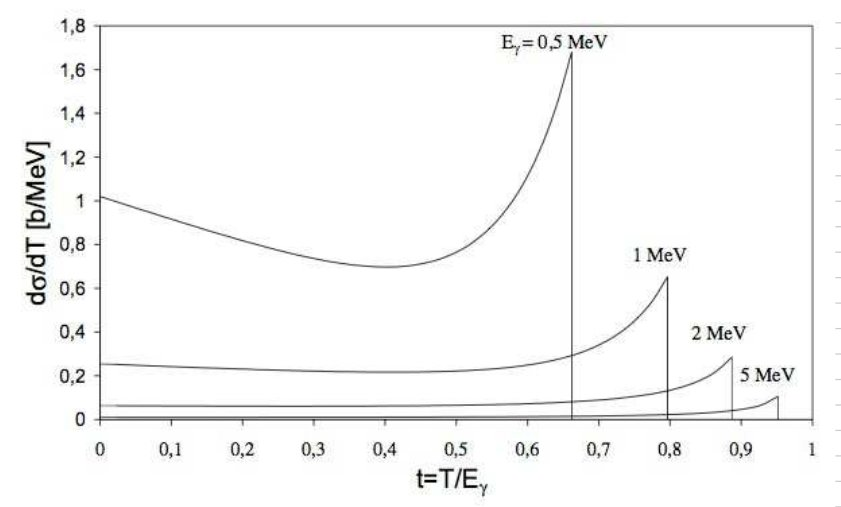
\includegraphics[width=0.5\textwidth]{10-comptonKante.jpg}
	\caption{	comptonTmax ???}
	\label{comptonTmax}
\end{figure}

Mit wachsendem $E$ gilt:

\[E_\gamma'(\Theta=\pi) \approx \frac{m_ec^2}{2}~~~~~\text{für}~~E_\gamma>>m_ec^2  \]

d.h. die Energie des gestreuten Photons entspricht der Hälfte der Elektronmasse.

% \section{Gasgefüllte Detektoren}
% \graphicspath{{bilder/3-1/}}
% Die relevanten Prozesse für den Energieverlust in gasgefüllten Detektoren sind Anregung und
Ionisation.
\\
Die Anregung eines Atoms $A$ durch ein geladenes Teilchen $x$ der Form

\[x+A \longrightarrow x+ A^*\]

erfordert eine genaue Energiemenge beim Übertrag. Typische Wirkungsquerschnitte liegen
im Bereich $\sigma_{\text{Anregung}}=10^{-17}\text{cm}^2$. Die Anregungsenergie kann über folgende Prozesse
abgegeben werden:

\begin{itemize}
  \item Strahlung:\\ $A^*\longrightarrow A+h\nu$
  \item Kollision:\\ z.B. $\text{Ne}^*+\text{Ar}\longrightarrow \text{Ne}+\text{Ar}^++e^-$
  \item Ion-Molekülbildung (Edelgase):\\ $\text{He}+\text{He} \longrightarrow\text{He}^+_2+e^-$
\end{itemize}

Die Ionisation eines Atoms $A$ der Form

\[x+A \longrightarrow x+ A^+ +e^- \]

erfordert dagegen keinen genauen Energieübertrag. Typischen Wirkungsquerschnitte liegen hierbei im
Bereich von $\sigma_{\text{Ion}}=10^{-16}\text{cm}^2$, was größer ist als
$\sigma_{\text{Anregung}}$. Da aber ein großer Energiebertrag erforderlich ist, um ein Atom zu
ionisieren, während kleine Energieüberträge häufiger sind, dominiert die Anregung über die Ionisation.
\\
Es gibt zwei Arten der Ionisation:

\begin{itemize}
  \item primäre Ionisation:\\ $x+A \longrightarrow x+A^++e^-$
  \item sekundäre Ionisation:\\ $x+A \longrightarrow x+A^++\delta_{e^-}$ \\ $\delta_{e^-}+A \longrightarrow
  x+A^++e^-$
\end{itemize}
% 	\subsection{Anzahl der Elektron-Ion-Paare}
% 		Der Energieverlust, der zur Ionisation nötig ist, ist größer als die Ionisationsenergie des Atoms.
Die mittlere Anzahl der Elektron-Ion-Paare ist gegeben durch

\[\frac{\text{Energieverlust des Teilchens}}{\text{mittlere Energie für die Erzeugung eines
$e^-$-Ion-Paares}} \]

Typische Werte für die benötigte Energie sind etwa $30\,$eV. So erzeugt ein $3\,$keV-Teilchen etwa
$\frac{3000\,\text{eV}}{30\,\text{eV}}=100$ $e^-$-Ion-Paare.

\begin{figure}[H]
	\centering
	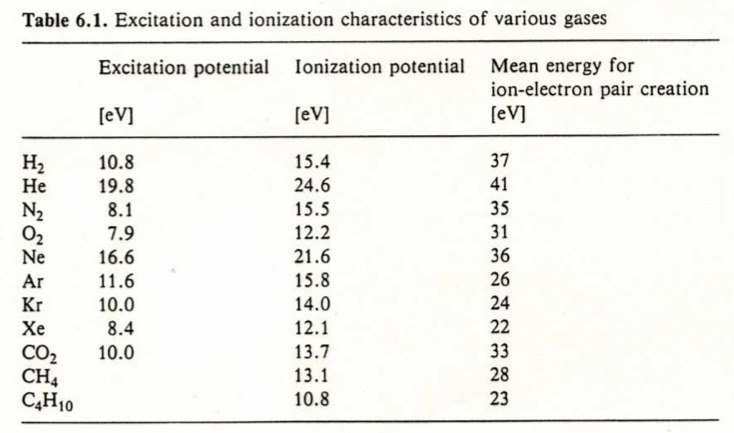
\includegraphics[width=0.75\textwidth]{Fig-03-01.jpg}
\end{figure}

Das Ziel ist die Bestimmung des Energieverlustes von Teilchen. Die Idee ist dabei, die Anzahl der
erzeugten $e^-$-Ion-Paare zu bestimmen - wobei gilt: je größer die Anzahl, desto genauer die
Messung.

\[\text{Teilchenenergie}\approx \#(\text{$e^-$-Ion-Paare})\cdot (\text{mittlere Energie für ein
$e^-$-Ion-Paar})\]

Für eine Anzahl $N_{\text{Mess}}\ge 20$ ergibt sich bei wiederholter Messung der erzeugten primären
Gesamtionisation ($N_{e^-/Ion}\cdot e$) eine Gaußkurve, wobei $\sigma_{\text{Q}}=$FWHM/2,35.

\begin{figure}[H]
	\centering
	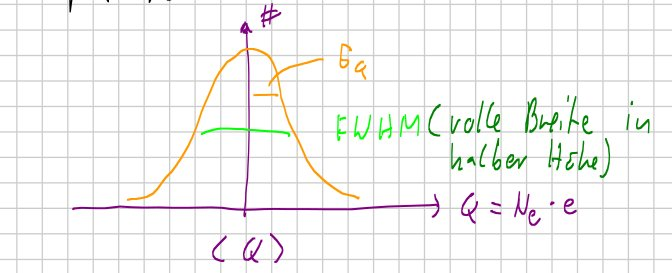
\includegraphics[width=0.5\textwidth]{gausskurve.jpg}
\end{figure}

Die relative Auflösung entspricht in diesem Fall

\[\frac{\sigma_{Q}}{\langle Q \rangle} =
\frac{\sqrt{N_{\text{Mess}}}}{N_{\text{Mess}}}=\frac{1}{\sqrt{N_{\text{Mess}}}}
\]

als bestmöglichste Auflösung für einen rein statistischen Prozess. Tatsächlich ergeben sich kleine
Werte, und zwar um den sogenannten Fano-Faktor $F$:

\[ F:=\frac{\text{beobachtete Auflösung}}{\text{erwartete Auflösung (aus Poisson-Statistik)}} \]

Beispiele:

\begin{description}
\item[$F=0{,}06$]: für Halbleiterzähler
\item[$F=1$]: für Szintillationszähler
\item[$F=0{,}2$]: für Edelgaszähler
\end{description}

Die Ionisationsprozesse sind nicht statistisch unabhängig!

% 	\subsection{Freie Ladungsträger in Gasen}
% 		Eine relevante Größe für die Beschreibung von Ladungsträgern in Gasen ist die Beweglichkeit $\mu$:

\[v_D = \mu\cdot E \cdot \frac{p_0}{p}  \]

mit dem Gasdruck $p$ und $p_0\approx 1013\,$mbar. $\mu$ ist die Proportionalitätskonstante zwischen
dem elektrischen Feld $E$ und der mittleren Geschwindigkeit $v_D$ des Ladungsträgers, der
sogenannten Driftgeschwindigkeit, die dieser im Feld $E$ erreicht.
\\
Bei Gasgemischen gilt:

\[\frac{1}{\mu_{i^+}} = \sum_{k=1}^n \frac{c_k}{\mu_{i^+_k}}  \]

wobei $c_k$ der Volumenkonzentration des Gases $k$ entspricht und $\mu_{i^+_k}$ der Beweglichkeit
des Ions der Sorte $i$ im Gas $k$.

\begin{figure}[H]
	\centering
	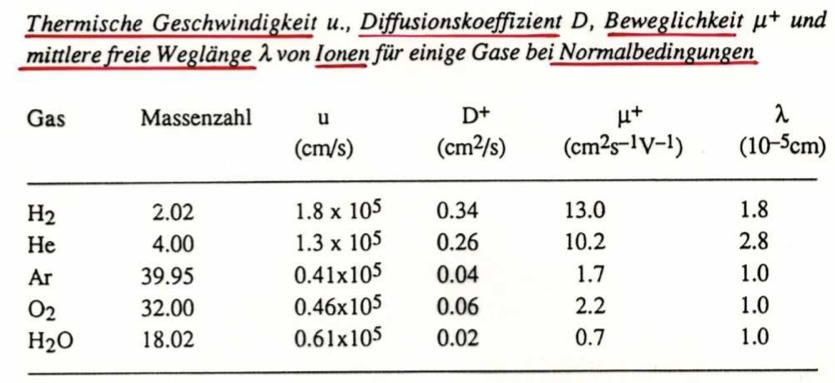
\includegraphics[width=0.75\textwidth]{Fig-03-02.jpg}
\end{figure}

\begin{figure}[H]
	\centering
	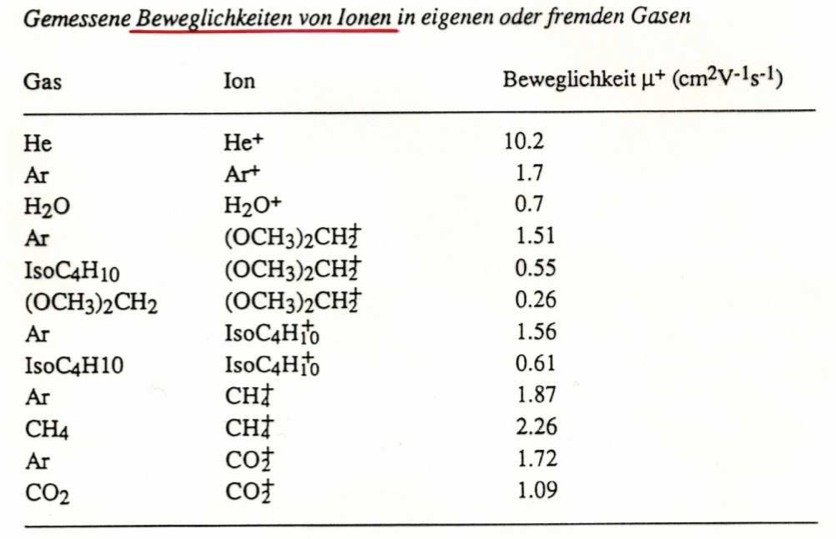
\includegraphics[width=0.75\textwidth]{Fig-03-03.jpg}
\end{figure}

\begin{figure}[H]
	\centering
	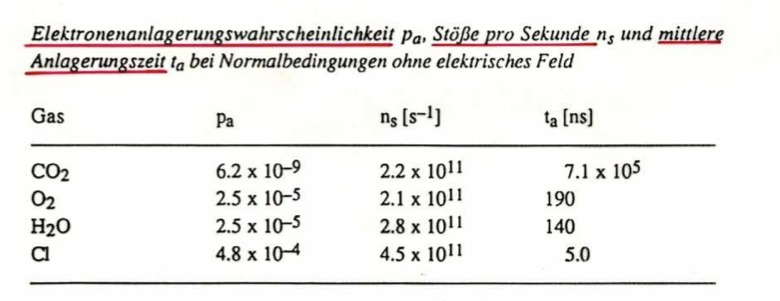
\includegraphics[width=0.75\textwidth]{Fig-03-04.jpg}
\end{figure}


% 	\subsection{Freie Ladungsträger in Gasen: Diffusion}
% 		Auch ohne äußere elektrische Felder bewegen sich freie Ladungsträger im Gas aufgrund ihrer
thermischen Energie. Diese Bewegung entspricht einer Maxwell-Verteilung. Für Ionen gilt

\[\langle E_{\text{kin}} \rangle = \frac{1}{2} m \langle u^2 \rangle ~~~~~\text{mit}~~~~ \langle u^2
\rangle = \frac{3kT}{m}
\]

Ausgangspunkt ist eine punktförmige Ladungsverteilung, die in eine zerfließende Gaußverteilung
übergeht.

\begin{figure}[H]
		\centering
		\includesvg[svgpath=bilder/3/]{punktzugauss}
\end{figure}

Dieser Prozess wird beschrieben durch

\[\frac{\mathrm{d}N}{N} = \frac{1}{\sqrt{4\pi\cdot D\cdot t}}\,
\text{exp}\left(-\frac{x^2}{4\,D\cdot t}\right)\,\mathrm{d}x
\]

wobei die Breite $\sigma_x=\sqrt{2D\cdot t}$ durch den Diffusionskoeffizienten $D$ beschrieben wird.
Je schneller die Teilchen sind, desto größer wird $D$. Insbesondere nimmt $\langle u^2 \rangle \sim
\frac{1}{m}$ mit abnehmender Teilchenmasse zu.
\\
Die mittlere freie Weglänge während des Diffusionsprozesses ist 

\[\lambda(E_{\text{kin}}) = \frac{1}{\frac{N_0\cdot\rho}{A}\cdot \sigma(E_{\text{kin}})} ,\]

also eine Funktion der kinetischen Energie des geladenen Teilchens.
\\
Die zuvor angegebene Breite der Gaußverteilung galt für die Diffusion in einer Dimension. In drei
Dimensionen gilt

\[\sigma = \sqrt{6D\cdot t} . \]

Der Diffusionskoeffizient kann in der kinetischen Gastheorie berechnet werden:

\[D=\frac{1}{3} \langle u \rangle \cdot \lambda~~~~~\text{mit}~~~~\langle u \rangle
=\sqrt{\frac{8\,k\cdot T}{\pi\cdot m}}\]

und $\lambda$ als mittlere freie Weglänge des Ladungsträgers. Damit ergibt sich das folgende Bild
für die expliziten Abhängigkeiten von $D$:

\[ D= \frac{2}{3\sqrt{\pi}}\cdot \frac{1}{\rho\cdot\sigma_0}\sqrt{\frac{(k\cdot T)^3}{m}} \]

\begin{itemize}
  \item $D\sim 1/\sqrt{m}$
  \item $D\sim \sqrt{T^3}$
  \item $D\sim 1/\rho$
\end{itemize}

Dabei ist $\sigma_0$ der totale Stoßwirkungsquerschnitt des Ladungsträgers mit einem Gasmolekül.
% 	\subsection{Rekombination und Elektronanlagerung}
% 		Das Ziel von Gasdetektoren ist die Messung bzw. Zählung der $e^-$-Ion-Paare. Ein Problem dabei
ergibt sich aus der Reduktion der Anzahl der $e^-$-Ion-Paare durch Rekombination und
Elektronanlagerung.
\\
Die Rekombination erfolgt nach dem Schema

\[A^+ + e^- \longrightarrow A + h\nu \]
\[A^+ + B^- \longrightarrow AB + h\nu  \]

Die Rekombinationsrate $dn$ hängt von den Konzentrationen des positiven ($n^+$) und negativen
($n^-$) Teilchen ab:

\[dn= \text{const}\cdot n^+ n^- \mathrm{d}t \]

Wenn $n^+=n^-\equiv n$ ist, dann folgt

\[n(t) = \frac{n_0}{1+\text{const}\cdot n_0\cdot t}  \]

\begin{figure}[H]
	\centering
	
\includegraphics[width=0.5\textwidth]{dummy.jpg}
\end{figure}

Eine Aufgabe bei der Konstruktion einer Detektors ist also, eine möglichst schnelle Trennung von
positiven und negativen Ladungen aus der Ionisation herbeizuführen.
\\
Bestimmte Atome bzw. Moleküle haben eine große Elektronenaffinität, beispielsweise wenn nur wenige
Elektronen zum Abschluss einer Schale fehlen. Diese stellen regelrechte "`Fallen"' für
freie Elektronen im Gas dar. Beispiele sind O$_2$, Cl$_2$, NH$_3$, H$_2$O, CCl$_4$ oder SF$_6$.
\\
Andere Gase (N$_2$, H$_2$, CH$_4$) haben vernachlässigbare oder sogar negative
Elektronenaffinität (Edelgase). Zudem hängt die Anlagerungswahrscheinlichkeit von der $e^-$-Energie
ab.

\begin{figure}[H]
	\centering
	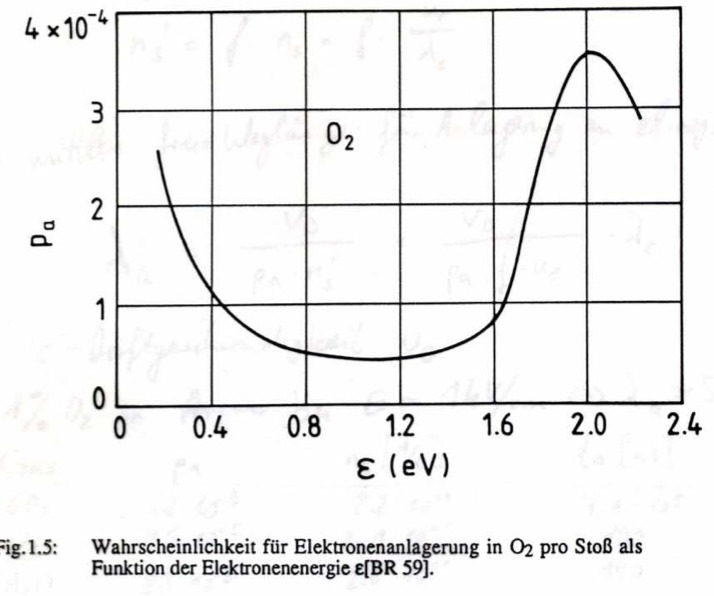
\includegraphics[width=0.5\textwidth]{Fig-03-05.jpg}
\end{figure}

Aus der thermischen Geschwindigkeit der Elektronen 

\[u_e = \sqrt{\frac{8kT}{\pi m}}  \]

und der mittleren freien Weglänge der Elektronen $\lambda_e \approx 4\cdot \lambda_{\text{Ion}}$
ergibt sich die Anzahl der Stöße pro Zeitintervall $n_S$:

\[ n_S = \frac{u_e}{\lambda_e}  \]

und daraus die Anlagerungswahrscheinlichkeit $p_a$ pro Stoß die mittlere Zeit bis zur Anlagerung

\[t_a=\frac{1}{p_a\cdot n_S}  .\]

Wenn elektronegative Moleküle mit dem Anteil f im Gas vorliegen, reduziert sich die Stoßrate zu

\[n_S' = f\cdot n_S = f\cdot \frac{u_e}{\lambda_e} \]

und für eine Driftgeschwindigkeit $v_D$ der Elektronen folgt als mittlere Weglänge bis zu Anlagerung

\[\lambda_a = \frac{v_D}{p_a\cdot n_S'}=\frac{1}{p_a\cdot f}\cdot \frac{v_D}{u_e}\cdot \lambda_e  
.\]

Beispiel: 1\% O$_2$ in Argon ergibt bei einer Driftfeldstärke von $E=1\,$keV/cm etwa
$\lambda_a\approx5\,$cm, was einen Verlust von Elektronen bei großen Driftdistanzen bedeutet.
% 	\subsection{Elektronendrift in elektrischen Feldern}
% 		Die große freie Weglänge $\lambda$ ermöglicht den Elektronen, anders als den Ionen, erhebliche
Energie im elektrischen Feld zu gewinnen. Im elektrischen Feld erreichen Elektronen Energien von
einigen keV, sodass ihre deBroglie-Wellenlänge im Bereich der Atomdurchmessers liegt.
Quantenmechanische Interferenzeffekte führen zu starken Abhängigkeiten des Stoßquerschnitts $\sigma$
von der kinetischen Energie der Elektronen und damit auch der freien Weglänge $\lambda\approx
1/\sigma$.

\begin{figure}[H]
	\centering
	
\includegraphics[width=0.5\textwidth]{dummy.jpg}
\end{figure}

Zur Herleitung einer Abschätzung der Driftgeschwindigkeit von Elektronen unter Einwirkung eines
elektrischen Feldes sei eine Gruppe von Elektronen mit thermischer Geschwindigkeit von

\[u=\sqrt{\frac{2E_{\text{kin}}}{m}}  \]

gegeben, die sich isotrop von einem Punkt $P$ fortbewegen:

\begin{figure}[H]
	\centering
	
\includegraphics[width=0.5\textwidth]{dummy.jpg}
\end{figure}

Unter Einwirkung eines elektrischen Feldes $\vec{E}$ werden aus den radialen Bahnen parabolische
Wege (Beschleunigung $\vec{b}=q\vec{E}/m$).

\begin{figure}[H]
	\centering
	
\includegraphics[width=0.5\textwidth]{dummy.jpg}
\end{figure}

$\delta_z$ ist die Verschiebung von $D+D_E$ entlang der z-Achse.
\\
Die Mittelung über alle cos$\,\Theta$ ergibt

\[ \langle \delta_z \rangle = \frac{1}{3}\cdot \frac{qE}{m}\cdot \langle t^2 \rangle \]

Für $\langle t^2 \rangle$ folgt durch die Mittelung der Laufzeiten über alle freien Weglängen $s$
und der thermicshen Elektronengeschwindigkeit $u$:

\[ \langle t^2 \rangle = \frac{\langle s^2 \rangle}{u^2} = \frac{2\lambda_e^2}{u^2} ,\]

wobei angenommen wurde, dass $\lambda_e$ unabhängig von $u$ ist (d.h. der Stoßquerschnitt $\sigma$
ist unabhängig von $u$). Damit ergibt sich als Driftgeschwindigkeit ($\langle t
\rangle=\lambda_e/u$):

\[v_D = \frac{\langle \delta_z \rangle}{\langle t\rangle} = \frac{2}{3}\cdot \frac{qE}{m}\cdot
\frac{\lambda_e}{u}\]

Zu berücksichtigen ist noch, dass die thermische Geschwindigkeit $u$ der Maxwell-Verteilung folgt.
Wird noch darüber gemittelt, so folgt

\[v_D\approx 0{,}92\cdot \frac{qE}{m}\cdot \frac{\lambda_e}{\sqrt{\langle
u^2\rangle}}~~~~~\text{mit}~~~~ \langle u^2\rangle = \frac{3kT}{m}\]

Zu beachten ist, dass $\lambda\sim \frac{1}{\text{Druck }p}$. Somit hängt $v_D$ explizit von der
reduzierten Feldstärke $E/p$ ab.
\\
Eine konstante Driftgeschwindigkeit erfordert, dass der Energiegewinn im $E-$Feld gleich
dem Energieverlust durch Stöße ist:

\[qE\cdot v_D\cdot \tau = \Delta(E_\text{kin})\cdot E_\text{kin}  \]

mit der Zeit $\tau$ zwischen zwei Stößen und dem Bruchteil der Energie $\Delta(E_\text{kin})$, die
beim Stoß auf das Gasatom übertragen wird. Es folgt

\[qE\cdot v_D = \frac{\Delta(E_\text{kin})\cdot E_\text{kin}}{\tau} =
\frac{\Delta(E_\text{kin})\cdot E_\text{kin}\cdot u}{\lambda_e}  \]

Für die konstante mittlere Driftgeschwindigkeit folgt dann weiterhin

\[qE\cdot v_D = \left\langle \frac{\Delta(E_\text{kin})\cdot E_\text{kin}}{\tau} \right\rangle =
\left\langle \frac{\Delta(E_\text{kin})\cdot E_\text{kin}\cdot u}{\lambda_e}\right\rangle \]

Um einige (quantitative) Aussagen über die Abhängigkeit der Driftgeschwindigkeit von der
elektrischen Feldstärke zu erhalten, sei im folgenden vereinfachend eine $\delta$-förmige
Geschwindigkeitsverteilung der für thermische Geschwindigkeit $u$ angenommen:

\[ E_\text{kin} = \frac{1}{2}\, m \cdot u^2 ~~~~~\Rightarrow ~~~~~ qE\cdot v_D\, \simeq\,
\frac{1}{2}\cdot \frac{\Delta(E_\text{kin})\cdot m\cdot u^3}{\lambda_e} , \]

sodass nach der Eliminierung von $u$ mittels 

\[v_D = \frac{2}{3} \cdot \frac{qE}{m}\cdot \frac{\lambda_e}{u} \]

gilt:

\[v_D \approx \sqrt{\frac{2}{3}\sqrt{\frac{\Delta(E_\text{kin})}{3}}\cdot \frac{qE}{m}\cdot\lambda_e} 
\]

Für die mittlere freie Weglänge $\lambda_e$ und den aufs Gasatom übertragenen Energiebruchteil
$\Delta(E_\text{kin})$ können als Näherung Potenzgesetze benutzt werden (vlg.
$\sigma-us-E$???-Diagramm und $\lambda_e\sim1/\sigma$):

\[\lambda_e(E_\text{kin})\sim E_\text{kin}^{-n}  \]
\[$\Delta(E_\text{kin})\sim E_\text{kin}^{+m} \]

Aus der Eliminierung von $E_\text{kin}=\frac{1}{2}\,m\cdot u^2$ in $v_D = \frac{2}{3} \cdot
\frac{qE}{m}\cdot \frac{\lambda_e}{u}$ und $qE\cdot v_D\cdot \tau = \Delta(E_\text{kin})\cdot
E_\text{kin}\cdot \frac{u}{\lambda_e}$ ergibt sich

\[v_D \sim E ^{(m+1)/(m+2n+1)}  \]

Dies bedeutet für die Kurve $\sigma-us-E$??? von Argon:

\begin{itemize}
  \item $E$ liegt unterhalb des Ramsauer-Minimums: $n\approx -1$\\
  $\rightarrow (m+1)/(m+2n+1)\approx \frac{m+1}{m-1}$\\
  $\rightarrow$ für $m\gtrsim 1$ wird der Exponent groß, d.h. $v_D$ steigt schnell mit der
  Feldstärke $E$ an.
  \item $E$ liegt oberhalb des Ramsauer-Minimums: $n\approx +1$\\
  $\rightarrow (m+1)/(m+2n+1)\approx \frac{m+1}{m+3}$\\
  $\rightarrow$ für $m\gtrsim 1$ ist der Exponent $\ge1/2$, d.h. $v_D$ steigt nur noch geringfügig
  mit der Feldstärke $E$ an.
\end{itemize}

Im Falle molekularer Gase wie CO$_2$, CH$_4$ \ldots existieren Schwingungs- und Rotationsanregungen
bei recht geringen Energien. Diese Anregungen tragen stark zum gesamten Stoßquerschnitt bei, wobei
der übertragene Energieanteil $\Delta(E_\text{kin})$ sehr groß wird, um dann oberhalb der maximalen
Schwingungsenergie $E_\text{max}$ rasch abzunehmen.

\[\Delta(E_\text{kin}) \sim \frac{E_\text{max}}{E_\text{kin}}  \]

Für $E_\text{kin}>E_\text{max}$ ist $m\simeq 1$, d.h. $(m+1)/(m+2n+1)\approx 0$ und somit ist dort
$v_D=\,$const (z.B. für Ethen C$_2$H$4$).
\\
Im Falle, dass $\Delta(E_\text{kin})$ stärker als $1/E_\text{kin}$ abnimmt, wird $m<-1$, sodass
$v_D$ mit der elektrischen Feldstärke $E$ sogar wieder abnimmt (z.B. für CH$_4$). Daher können schon
kleine Verunreinigungen mit molekularen Gasen zu starken Veränderungen der Driftgeschwindigkeiten
führen.

\begin{figure}[H]
	\centering
	
\includegraphics[width=0.5\textwidth]{dummy.jpg}
\end{figure}

\begin{figure}[H]
	\centering
	
\includegraphics[width=0.5\textwidth]{dummy.jpg}
\end{figure}
% 	\subsection{Elektronendrift in elektrischen und magnetischen Feldern}
% 		Zusätzlich zur Coulombkraft $q\vec{E}$ wirkt nun auch noch die Lorentzkraft $q\vec{v}\times
\vec{B}$. Unter alleiniger Wirkung eines $B$-Feldes vollführt ein geladenes Teilchen eine
Kreisbewegung mit der Frequenz

\[\vec{\omega} = -\frac{q\vec{B}}{m}\]

mit der Elektron-Zyklotronfrequenz $\vec{\omega}$ und
$\frac{\omega}{B}=17{,}6\,\frac{\text{MHz}}{\text{Gauß}}$. Treten $\vec{E}$- und $\vec{B}$-Felder
gemeinsam auf, kann die dann schraubenförmige Bewegung in eine Rotationsbewegung mit Kreisfrequenz
$\omega$ und eine Translationsbewegung mit Geschwindigkeit $v_D$ zerlegt werden
($\vec{r}\,\perp\,\vec{v}_D$). 

\begin{figure}[H]
	\centering
	
\includegraphics[width=0.5\textwidth]{dummy.jpg}
\end{figure}

\[ \vec{v}= \vec{v}_D + \vec{\omega}\times\vec{r} \]
 
 mit
 
 \[\vec{v}_D=\vec{E}\times \vec{B}/\beta^2 +\vec{v}_\shortparallel  \]
 \[\dot{\vec{v}}_\shortparallel = \frac{q}{m} \cdot\vec{E}_\shortparallel\]
 
 wobei $\vec{v}_\shortparallel$ und $\vec{E}_\shortparallel$ die Komponenten parallel zu $\vec{B}$
 sind.
 \\
 In Gasen kommet es zudem zu Stößen mit den Gasmolekülen, d.h. man muss die stochastische Kraft
 "`$m\cdot\vec{a}(t)$"' berücksichtigen. Dies führt zu der Bewegungsgleichung:
 
 \[m\cdot \dot{\vec{v}} = q\left( \vec{E}+\vec{v}\times\vec{B} \right) +m\cdot
 \vec{a}(t)~~~~~~~~~~\text{Langevin-Gleichung} \]

 Im zeitlichen Mittel gilt
 
 \[\langle \vec{a}(t) \rangle = - \dot{\vec{v}}_D  \approx \frac{\vec{v}_D}{\tau}. \]
 
 Im zeitlichen Mittel muss aus der Gleichung die Translationsbewegung mit konstanter
 Driftgeschwindigkeit folgen, d.h. die stochastische Beschleunigung $\vec{a}$ muss im Mittel gerade
 die translatorische Beschleunigung $\dot{\vec{v}}_D$ kompensieren.
% 	\subsection{Gasverstärkung}
% 		Bisher wurden nur geringe $\vec{E}$-Felder betrachtet, womit der Energiegewinn der Elektronen klein
ist ($qE\lambda_e$). Sehr starke Felder ermöglichen dagegen einen Energiegewinn, der eine
Sekundärionisation möglich macht. Daraus folgt eine Zunahme der Ladungsträger.

\begin{figure}[H]
	\centering
	
\includegraphics[width=0.5\textwidth]{dummy.jpg}
\end{figure}

Diese lawinenartige Zunahme führt zu einer erheblichen Ladungsmenge, die einfach gemessen werden
kann. Man nennt diesen Prozess Gasverstärkung.
\\
Die Anzahl der Elektron-Ion-Paare, die ein Elektron pro cm Wegstrecke bildet, wird durch den ersten
Townsend-Koeffizienten $\alpha$ bezeichnet. Aus dem Stoßquerschnitt $\sigma_i$ kann $\alpha$ durch 

\[\alpha = \sigma_i\cdot N~~~~~~\text{mit}~~~~~ N=\frac{N_0}{V_{\text{mol}}}\approx
2{,}69\cdot10^{19}\,\frac{\text{Atome}}{\text{cm}^3} \]

berechnet werden. Eine Elektronenlawine hinterlässt eine charakteristische Verteilung der positiven
und negativen Ladungsträgern in Tropfenform. Die höhere Beweglichkeit der Elektronen führt zu der
"`negativen"' Spitze (siehe Abb. \ref{bla}). Die eigentliche Tropfenform entsteht durch die
unbeweglichen Ionen.

\begin{figure}[H]
	\centering
	
\includegraphics[width=0.5\textwidth]{dummy.jpg}
\end{figure}

Beginnend mit $n_o$ Primärelektronen am Ort $x=0$ werden durch Stoßionisation entlang von $dx$

\[ dn = \alpha\cdot n \mathrm{d}x  \]

zusätzliche Elektronen erzeugt, sodass

\[n(x)=n_0\cdot e^{\alpha\cdot x}   \]

gilt, falls $\alpha$ unabhängig von $x$ ist. Da $\alpha$ von der Feldstärke abhängt, die sich
entlang von $x$ ändern kann, gilt

\[n(x)=n_0\cdot \text{exp}\left(\int\alpha(x)\mathrm{d}x \right)=:n_0\cdot A  .\]

Dabei bezeichnet $A$ die Gastverstärkung. $A$ hängt von der freien Weglänge $\lambda$ ab:

\[\lambda =\frac{1}{\alpha}=\frac{1}{N\cdot\sigma_i}  \]

Wichtig ist hierbei: Die Anzahl der Elektronen am Ort $x$ ist proportional zu $n_0$
(Proportionalitätsbereich der Gasverstärkung).
\\
Das Ende des exponentiellen Anstiegs der Gasverstärkung wird durch UV-Photonen eingeleitet, die
durch den Photoeffekt im Gas oder aus der Kathode weitere Elektronen auslösen.

\[n_0 \text{ primäre Elektronen} \longrightarrow A\cdot n_0 \text{ Elektronen} + (A\cdot n_0)\cdot
\gamma \text{ Photoelektronen}\]
\[(A\cdot n_0)\cdot\gamma \text{ Photoelektronen} \longrightarrow A(A\cdot n_0)\cdot \gamma
\text{ Elektronen} + A(A\cdot n_0)\cdot \gamma^2 \text{ Photoelektronen}\]
\ldots

Hierbei bezeichnet $\gamma$ den zweiten Townsend-Koeffizenten.

Die Gasverstärkung einschließlich der Energieausbreitung durch Photonen ist


\begin{align*}
A_\gamma :&= n_0\cdot A + n_0\cdot A^2\cdot\gamma + n_0\cdot A^3\cdot\gamma^2 + \ldots\\
&=n_0\cdot A \sum_{\nu\geq0}(A\cdot\gamma)^\nu  \\
&= \frac{n_0\cdot A}{1- A\cdot\gamma}
\end{align*}

wenn $A\cdot\gamma<1$. Somit ist $A_\gamma\sim n_0$.
\\
Für $A_\gamma\rightarrow 1$ wird $A\gamma$ unabhängig von $n_0$. In diesem sogenannten
Auslösebereich wird $\alpha\cdot x\approx 20$ oder $A\approx10^8$ erreicht.

\begin{figure}[H]
	\centering
	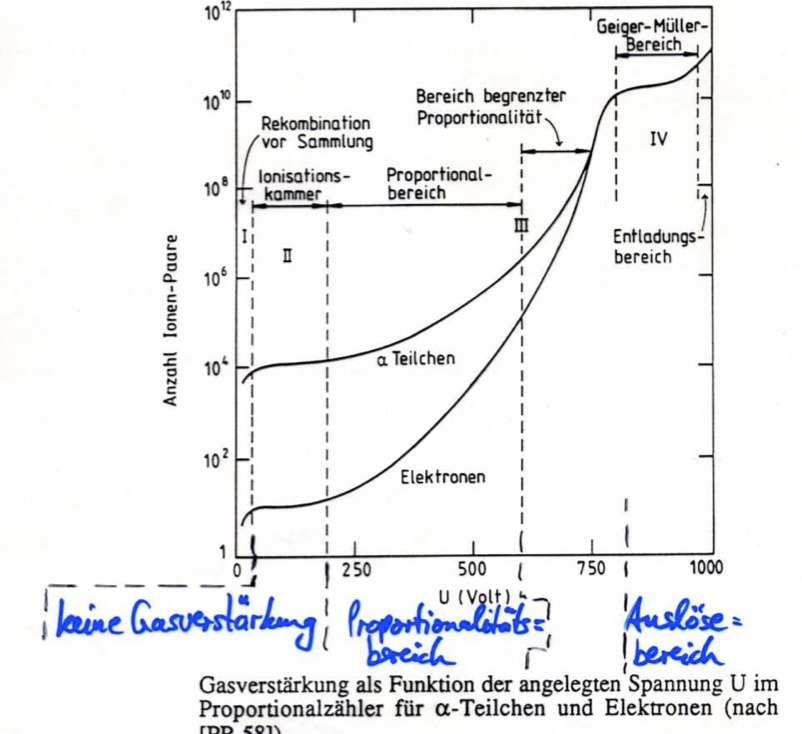
\includegraphics[width=0.65\textwidth]{Fig-03-16.jpg}
	\caption{Abhängig von der $|\vec{E|}$-Feldstärke können verschiedene Bereiche der Gasverstärkung
	identifiziert werden.}
\end{figure}

\subsubsection*{Berechnung erster Townsend-Koeffizient}

Eine einfache, für kleine $\alpha$ gültige Approximation des ersten Townsend-Koeffizienten $\alpha$
stammt von S. Korff:

\[\alpha \approx p\cdot A\cdot e^{-\beta p/E}  \]

mit dem Druck $p$ und der Feldstärke $E$. In diesem Bereich ist $\alpha$ zudem linear abhängig von
der kinetischen Elektronenergie $E_\text{kin}$

\[\alpha \approx k\cdot N \cdot E_\text{kin} ~~~~~~ \text{mit}~~~~~N\approx 2{,}69\cdot
10^{19}\,\frac{\text{Atome}}{\text{cm}^3}.\]

Die Parameter $A, \beta$ und $k$ sind z.B.:

\begin{figure}[H]
	\centering
	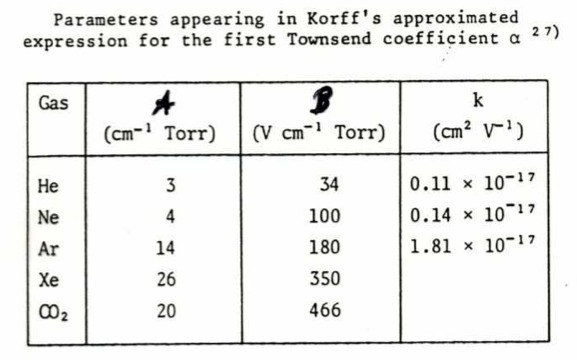
\includegraphics[width=0.5\textwidth]{Fig-03-17.jpg}
\end{figure}

\subsubsection*{Zusammenfassung}

Ionisation und Anregung erzeugen freie Ladungsträger im Gas. Diese Ladungsträger können sich durch
Diffusion oder unter der Wirkung elektrischer Felder im Gas gemäß ihrer Beweglichkeit $\mu$
bewegen. Elektronegative Atome lagern dabei freie Elektronen an. Im elektrischen Feld stellt sich
eine konstante Driftgeschwindigkeit $v_D\sim E\lambda_e/T$ ein, ihr Wert hängt vom
Elektron-Gasatom-Stoßwirkungsquerschnitt ab (Ramsauer-Minimum). Im elektrischen und magnetischen
Feld ergibt sich eine schraubenförmige Bewegung. Diese Felder beeinflussen auch die Diffusion.
\\
Sehr starke elektrische Felder führen zur Gasverstärkung mit leicht messbaren Ladungsmengen.
				
				
\end{document}